\chapter{SQL}

\begin{introduction}[期末考试提纲]
  \item 了解数据类型、表的定义
  \item 掌握各种索引的定义及其作用
  \item 掌握各种查询表达操作的含义
  \item 能用SQL表达查询操作
  \item 表连接、分组聚集、集合、嵌套子查询、null、游标、with定义临时视图
\end{introduction}

SQL: Structured Query Languang

SQL语言的特点:
\begin{enumerate}
    \item 语言简洁,易学易用。
    \item 面向集合的操作方式,一次一集合。
    \item 高度非过程化。\textit{用户只需提出“做什么” ,无须告诉“怎么做”}
    \item 一体化。单一的结构——关系,带来了数据操作符的统一。
    \item 两种使用方式,统一的语法结构。
    \begin{enumerate}
        \item 既是自含式(用户使用)的
        \item 又是嵌入式的(程序员使用)
    \end{enumerate}
\end{enumerate}

\begin{table}[H]
  \centering
  \begin{tabular}{|c|c|}
    \hline
    \textbf{SQL功能} & \textbf{操作符} \\
    \hline
    数据定义 & \verb|create|, \verb|alter|, \verb|drop| \\
    \hline
    数据查询 & \verb|select| \\
    \hline
    数据修改 & \verb|insert|, \verb|update|, \verb|delete| \\
    \hline
    数据控制 & \verb|grant|, \verb|revoke| \\
    \hline
  \end{tabular}
  \caption{SQL主要操作符}
\end{table}

text2SQL: 建立自然语言与结构化数据之间的关系。

\section{数据定义}

\begin{figure}[H]
  \centering
  \begin{minipage}[t]{0.45\textwidth}
    \centering
    \includegraphics[width=\linewidth]{./figure/标准SQL.pdf}
    \caption{标准SQL中的数据定义对象}
  \end{minipage}
  \hfill
  \begin{minipage}[t]{0.5\textwidth}
    \centering
    \includegraphics[width=\textwidth]{./figure/实际.pdf}
    \caption{实际数据库(SQL Server)中的定义对象}
  \end{minipage}
\end{figure}

SQL Server: 模式把对象和用户分离开来.

对象命名: \verb|<数据库>.<模式>.<表>|.

\subsection{数据模式定义}

创建模式:
\begin{lstlisting}[language=SQL]
create schema <模式名>
create schema University.Library
\end{lstlisting}

数据库定义: SQL Server
\begin{lstlisting}[language=SQL]
create database <数据库名>
  [on [primary] <文件描述> <文件组> ...]
  [log on <文件描述> <文件组> ...]
\end{lstlisting}

最简单的创建数据库的命令: \verb|create databse University|.

\verb|use| 命令指定当前要使用的数据库: \verb|use University|.

\begin{lstlisting}[language=SQL]
create database demoDB1
on primary
( name = demo_dat1,
  filename = 'D:\SQL_Practice\demodata1.mdf',
  size = 10,
  maxsize = 50)
log on
(
  name = demo_log1,
  filename = 'D:\SQL_Practice\demodata1.ldf',
  size = 5,
  filegrowth = 5
)
\end{lstlisting}

数据库定义: MySQL
\begin{lstlisting}[language=SQL]
create database <数据库名>
  [ default character set utf8
    default collate utf8_Chinese_ci ]
\end{lstlisting}

\verb|create database| 等于 \verb|create schema|.

MySQL表空间:

\begin{figure}[H]
    \centering
    \includegraphics[width=.45\textwidth]{./figure/MySQL表空间.pdf}
    \caption{MySQL表空间}
\end{figure}

\begin{lstlisting}[language=SQL]
create tablespace myTs 'ts1.ibd' engine = innodb
create tablespace myTs add datafile
  'F:\\test_mysql_tablespace\\first.ibd'
create table myTb (...) tablespace myTs
\end{lstlisting}

创建基本表的语法命令:
\begin{lstlisting}[language=SQL]
create table <表名> (
  <列名> <数据类型> [default <缺省值>] [not null] [unique]
  [, <列名> <数据类型> [default <缺省值>] [not null] [unique]]
  ...
  [, primary key (<列名> [, <列名>] ...)]
  [, foreign key (<列名> [, <列名>] ...)
    references <表名> (<列名> [, <列名>] ...)]
  [, check(<条件>)]
)
\end{lstlisting}

下面是创建表的一些例子:
\begin{lstlisting}[language=SQL]
create table student
( sno char(8),
  sname char(8) not null default '佚名',
  age tinyint,
  sex char(1),
  primary key (sno),
  check (sex = 'M' or sex='F')
)
\end{lstlisting}

\begin{lstlisting}[language=SQL]
create table course
( cno char(8) primary key,
  cname char(8) not null unique,
  pcno char(8) foreign key references C(cno),
  credit tinyint
)
\end{lstlisting}

\begin{lstlisting}[language=SQL]
create table SC
( sno char(8) foreign key references S(sno),
  cno char(8) foreign key references C(cno),
  grade tinyint,
  primary key (sno, cno),
  check((grade is null) or grade between 0 and 100)
)
\end{lstlisting}

修改基本表: 更改、添加、除去列和约束.
\begin{lstlisting}[language=SQL]
alter table <表名>
  [add column <子句>]
  [add constraint <子句>]
  [drop <子句>]
  [alter column <子句>]
\end{lstlisting}

\begin{lstlisting}[language=SQL]
-- 在student表age列之后加入addr
alter table student add column addr CHAR(30) after age;
-- 把addr列重命名为address
alter table student change addr address CHAR(50) not null;
-- 试修改teacher表中的salary列的数据类型为bigint
alter table teacher modify salary bigint;
-- 重命名一个表中的列名从sal到salary
alter table rename sal to salary
\end{lstlisting}

删除基本表:
\begin{lstlisting}[language=SQL]
drop table <表名>;
\end{lstlisting}
删除表定义及该表的所有数据、索引、触发器、约束和权限规范.

drop table不能删除被foreign key约束所引用的表, 必须先除去foreign key约束或引用表.

任何引用已删除表的视图或存储过程必须通过drop view或drop procedure语句显式除去.

标准SQL中的信息视图:
\begin{lstlisting}[language=SQL]
INFORMATION_SCHEMA.SCHEMATA
INFORMATION_SCHEMA.TABLES
INFORMATION_SCHEMA.COLUMNS
INFORMATION_SCHEMA.CHECK_CONSTRAINTS
INFORMATION_SCHEMA.VIEWS
INFORMATION_SCHEMA.DOMAINS
\end{lstlisting}

MySQL中的信息视图查询:
\begin{lstlisting}[language=SQL]
select shcema_name from information_schema.schemata;
select table_name from information_schema.tables;
select column_name from information_schema.columns where table_name = 'student';
\end{lstlisting}

\begin{table}[H]
\centering
\label{tab:sysobjects}
\begin{tabular}{|l|l|l|}
\hline
\multicolumn{3}{|c|}{sysobjects} \\ \hline
\textbf{列名} & \textbf{数据类型} & \textbf{描述} \\ \hline
name & sysname & 对象名 \\ \hline
Id & int & 对象标识号 \\ \hline
xtype & char(2) & 对象类型 \\ \hline
uid & smallint & 所有者对象的用户ID \\ \hline
crdate & datetime & 对象的创建日期 \\ \hline
schema\_ver & int & 版本号,该版本号在每次表的架构更改时都增加 \\ \hline
\end{tabular}
\caption{表定义相关的字典表: SQL Server}
\end{table}

\begin{table}[H]
\centering
\label{tab:syscolumns}
\begin{tabular}{|l|l|l|}
\hline
\multicolumn{3}{|c|}{syscolumns} \\ \hline
\textbf{列名} & \textbf{数据类型} & \textbf{描述} \\ \hline
name & sysname & 列名或过程参数的名称 \\ \hline
id & int & 该列所属的表对象ID \\ \hline
 xtype & tinyint & systypes 中的物理存储类型 \\ \hline
xusertype & smallint & 扩展的用户定义数据类型ID \\ \hline
length & smallint & systypes 中的最大物理存储长度 \\ \hline
offset & smallint & 该列所在行的偏移量;如果为负,表示可变长度行 \\ \hline
type & tinyint & systypes 中的物理存储类型 \\ \hline
usertype & smallint & systypes 中的用户定义数据类型ID \\ \hline
isnullable & int & 表示该列是否允许空值 \\ \hline
\end{tabular}
\caption{表定义相关的字典表: SQL Server}
\end{table}

SQL中, 任何时候都可以执行一个数据定义语句, 随时修改数据库结构.

\subsection{数据类型}

\begin{table}[H]
\centering
\label{tab:mysql_int_types}
\begin{tabular}{|l|l|l|l|}
\hline
\textbf{数据类型} & \textbf{范围} & \textbf{unsigned范围} & \textbf{存储字节数} \\ \hline
tinyint & $-2^7 \sim 2^7 - 1$ & $0 \sim 2^8 - 1$ & 1字节 \\ \hline
smallint & $-2^{15} \sim 2^{15} - 1$ & $0 \sim 2^{16} - 1$ & 2字节 \\ \hline
mediumint & $-2^{23} \sim 2^{23} - 1$ & $0 \sim 2^{24} - 1$ & 3字节 \\ \hline
int & $-2^{31} \sim 2^{31} - 1$ & $0 \sim 2^{32} - 1$ & 4字节 \\ \hline
bigint & $-2^{63} \sim 2^{63} - 1$ & $0 \sim 2^{64} - 1$ & 8字节 \\ \hline
\end{tabular}
\caption{MySQL整数数据类型及其范围和存储字节数}
\end{table}

\begin{lstlisting}[language=SQL]
create table test_int (
  a(6) tinyint zerofill,
  b(6) tinyint unsigned );
insert into test_int values (1, 111);
select a, b from test_int;
-- a 000001 b 111
select a - b from test_int;
-- ERROR 1690 (22003): BIGINT UNSIGNED value is out of range
\end{lstlisting}

宽松模式: \verb|set sql_mode = 'ANSI'|. 对于违反数据约束的有一些默认操作.

严格模式: \verb|set sql_mode = 'traditional'|. 直接报错.


\begin{table}[H]
  \centering
  \begin{tabular}{|l|l|l|l|}
    \hline
    \textbf{数据类型} & \textbf{描述} & \textbf{unsigned范围} & \textbf{存储字节数} \\ \hline
    \verb|float|($m$, $d$) & \makecell[l]{单精度浮点数\\ $m$是总位数\\ $d$是小数点后位数} & ... & 4字节 \\ \hline
    \verb|double|($m$, $d$) & \makecell[l]{双精度浮点数\\ $m$是总位数\\ $d$是小数点后位数} & ... & 8字节 \\ \hline
    \makecell[l]{\texttt{decimal}($m$, $d$) \\ \texttt{numeric}} & \makecell[l]{精确小数\\ $m$是总位数\\ $d$是小数点后位数} & \makecell[l]{最大位数$m$为65 \\ 最大支持小数为$d$为30} & \\ \hline
    \verb|float|($n$) & ... & ... & \makecell[l]{$1\leq n \leq 24$是4字节\\ $25\leq n \leq 53$是8字节} \\ \hline
  \end{tabular}
  \caption{定点数与浮点数}
\end{table}

money使用4位小数存储数据, 容易发生小数的舍入错误.

\begin{table}[H]
  \centering
  \begin{tabular}{|l|l|l|l|}
    \hline
    \textbf{数据类型} & \textbf{范围} & \textbf{描述} & \textbf{存储字节数} \\ \hline
    \verb|char|($n$) & $0\sim 255$ & 定长字符串 & 4字节 \\ \hline
    \verb|varchar|($n$) & $0\sim 65,535$ & 变长字符串 & 实际字符串长度 \\ \hline
    \makecell[l]{\texttt{tinytext} \\ \texttt{text} \\ \texttt{mediumtext}\\ \texttt{longtext}} & \makecell[l]{$0\sim 2^8$\\ $0\sim 2^{16}$\\ $0\sim 2^{24}$ \\ $0\sim 2^{32}$} &  & \\ \hline
  \end{tabular}
  \caption{字符型}
\end{table}

\begin{lstlisting}[language=SQL]
-- 创建表时指定字符集和校对规则
CREATE TABLE users (
  name VARCHAR(100)
) CHARACTER SET utf8mb4 COLLATE utf8mb4_unicode_ci;
-- ci 表示不区分大小写

-- 查看服务器字符集
SHOW VARIABLES LIKE 'character_set%';
-- 查看数据库字符集
SHOW CREATE DATABASE mydb;
-- 查看表字符集
SHOW CREATE TABLE users;
\end{lstlisting}

\begin{table}[H]
    \centering
    \begin{tabular}{|l|l|p{5cm}|l|}
        \hline
        \textbf{类型名称} & \textbf{日期格式} & \textbf{日期范围} & \textbf{存储需求} \\ \hline
        year & YYYY & 1901 $\sim$ 2155 & 1 个字节 \\ \hline
        time & HH:MM:SS & -838:59:59 $\sim$ 838:59:59 & 3 个字节 \\ \hline
        date & YYYY-MM-DD & 1000-01-01 $\sim$ 9999-12-31 & 3 个字节 \\ \hline
        datetime & YYYY-MM-DD HH:MM:SS & 1000-01-01 00:00:00 $\sim$ 9999-12-31 23:59:59 & 8 个字节 \\ \hline
        timestamp & YYYY-MM-DD HH:MM:SS & 1980-01-01 00:00:01 UTC $\sim$ 2040-01-19 03:14:07 UTC & 4 个字节 \\ \hline
    \end{tabular}
    \caption{日期类型及其描述}
    \label{tab:date_types}
\end{table}

\begin{table}[H]
  \centering
  \begin{tabular}{|l|l|}
    \hline
    \textbf{数据类型} & \textbf{描述} \\ \hline
    \verb|enum('v1', 'v2', ...)| & 只能取一个值 \\ \hline
    \verb|set('v1', 'v2', ...)| & 可以取多个值 \\ \hline
  \end{tabular}
  \caption{枚举型}
\end{table}

\begin{lstlisting}[language=SQL]
create table test_enum(
  a enum('男' ,'女'),
  b set('1', '2', '3', '4') )
insert into test_enum values ('男', '2,4')
\end{lstlisting}

\begin{table}[H]
  \centering
  \begin{tabular}{|l|l|}
    \hline
    \textbf{数据类型} & \textbf{大小} \\ \hline
    \verb|binary(n)| & 255 \\ \hline
    \verb|varbinary(n)| & 16384 \\ \hline
    \verb|tinyblob, blob, mediumblob, longblob| & 256, 16K, 16M, 4G \\ \hline
  \end{tabular}
  \caption{二进制类型}
\end{table}

下面是几个关于数据类型的问题:
\begin{enumerate}
    \item char 还是 varchar?
    \begin{table}[H]
      \centering
      \begin{tabular}{|l|l|l|}
        \hline
        \textbf{特性} & \textbf{CHAR} & \textbf{VARCHAR} \\ \hline
        存储方式 &	固定长度 & 可变长度 \\ \hline
        存储效率 & 可能浪费空间(固定长度填充空格) &	高效(仅存储实际数据 + 长度信息)\\ \hline
        检索速度 & 更快(直接定位)& 稍慢(需计算长度) \\ \hline
        适用场景 & 固定长度数据(如代码、哈希值) &	可变长度数据(如姓名、地址) \\ \hline
        空格处理 & 自动填充空格(需注意业务逻辑) &	不填充空格 \\ \hline
      \end{tabular}
    \end{table}
    \item 显式数据类型转换: 
    \begin{lstlisting}[language=SQL]
cast ( 表达式 as 数据类型 [(数据长度)] )
convert ( 数据类型 [(数据长度)], 表达式 [, 输出样式] )
select cast( 123.45 as decimal(10,4) )            -- 输出结果: 123.4500
select cast( 123.45 as decimal(10,1) )            -- 输出结果: 123.5
select cast( 12.34567 as money )                  -- 输出结果: 12.3457
select 'My age is: ' + cast( 28 as char(4) )      -- 输出结果: My age is: 28
select cast( cast( 123.45 as int ) as char(10) )  -- 输出结果: 123
select convert( varchar(30), getdate(), 106 )     -- 输出结果: 17 08 2012
select convert( varchar(30), getdate(), 110 )     -- 输出结果: 08-17-2012
select cast( 'SQL' as binary(3) )                 -- 输出结果: 0x53514C
    \end{lstlisting}
    \item 隐式数据类型转换: 执行\verb|select 1 + '1'|, 结果会是2; 执行\verb|select 1 + 'a'|, 会显示类型转换错误.
    \item 特殊类型: XML, JSON, Array, 空间数据.
    \item 用户定义数据类型UDDT(User-defined Datatype).
    \begin{itemize}
      \item 标准SQL: \verb|create domain 域名 数据类型|;
      \item SQL Server: \verb|create type phone_number from varchar(20) not null|.
      \item Oracle: 
      \begin{lstlisting}[language=SQL]
create type animal_ty as OBJECT(
  breed varchar2(25),
  name vharchar2(25),
  birthday date
)
      \end{lstlisting}
    \end{itemize}
    \item 冗长主码的危害: 占据很大的表空间; 减少索引项, 增加了磁盘I/O数, 减慢索引速度.
\end{enumerate}

MySQL中的自增字段:
\begin{lstlisting}[language=SQL]
create table test_incr(
  id bigint auto_increment,
  name char(10)
)
\end{lstlisting}

SQL Server中的序列号: identity.
\begin{lstlisting}[language=SQL]
create table customer(
  cust_id smallint identity(100, 20) not null,
  -- identity 有一个起始数和增量值
  cust_name varchar(50) not null
)
\end{lstlisting}

SQL Server中的序列号: sequence.
\begin{lstlisting}[language=SQL]
create sequence mySeq as int start with 1 increment by 1
insert into myTb(id, Name) values (next value for mySeq, 'Tom')
insert into myTb(id, Name) values (next value for mySeq, 'jerry')
\end{lstlisting}

uniqueidentifier 产生跨数据库和服务器的全局唯一标识符(GUID), newid()函数产生uniqueidentifier 类型的值, newsequentialid()产生的GUID总是大于先前通过该函数生成的GUID.

如果表中有一列被声明为rowversion, 只要行被修改, 其rowversion
列就会发生改变. 它是跨表唯一的, 任何表的修改都会使该值递增.

\subsection{索引}

\begin{definition}[索引]
  索引是数据库管理系统中用于加速数据检索的核心工具. 
  它通过创建特定数据结构(如B树、哈希表等), 
  将数据表中的某些列的值与对应的物理存储位置关联起来, 从而大幅提升查询效率.
\end{definition}

索引的作用:
\begin{itemize}
  \item 加速查询;
  \item 支持排序和分组;
  \item 保证唯一性;
  \item 优化连接操作.
\end{itemize}

\begin{lstlisting}[language=SQL]
create [unique] index 索引名
  [using { btree | hash }]
on 表名 (列名 [asc/desc] [, 列名asc/desc] ...)

drop index 索引名
\end{lstlisting}

\begin{figure}[H]
  \centering
  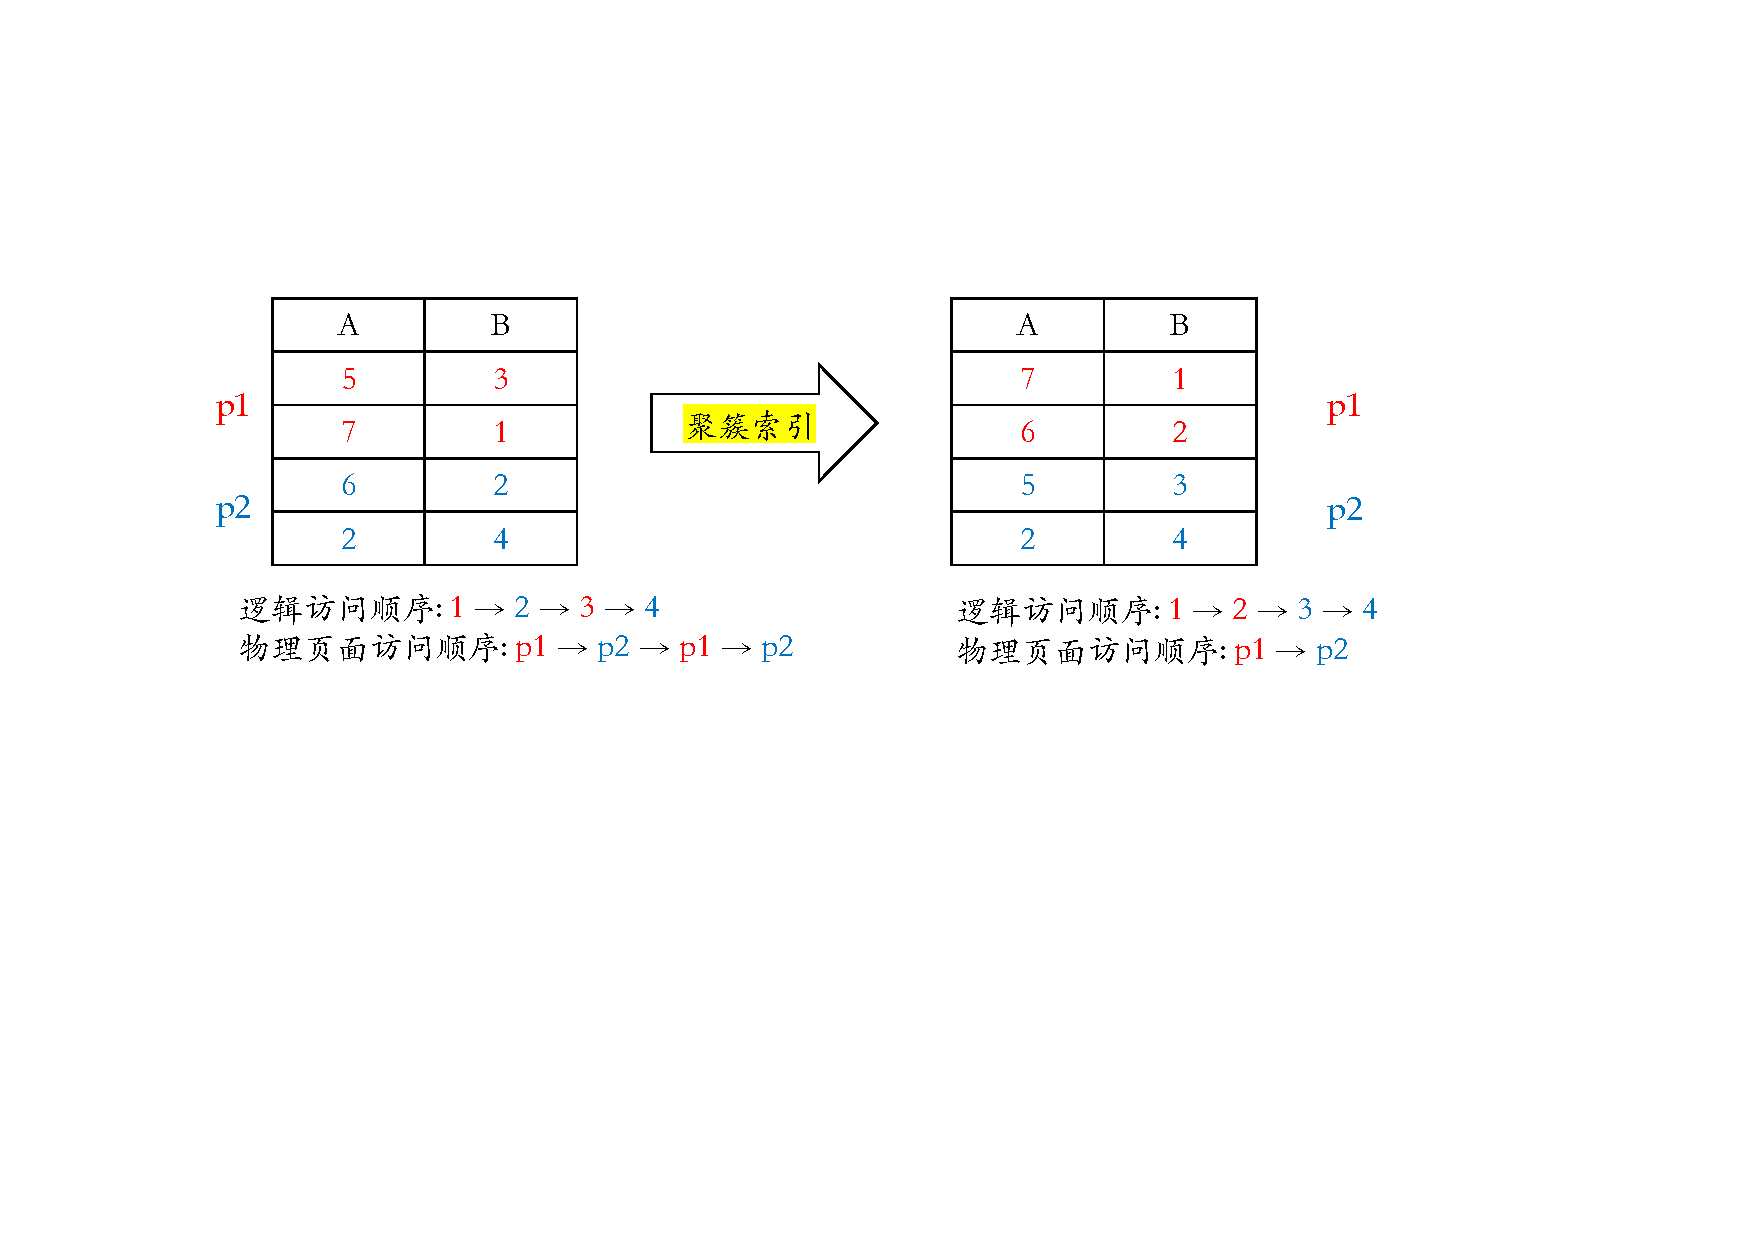
\includegraphics[width=.8\textwidth]{figure/聚簇索引.pdf}
  \caption{聚簇索引}
  \label{fig:cluster}
\end{figure}

\begin{definition}[索引碎片]
  索引碎片: 页面逻辑顺序与物理顺序不一致.
\end{definition}

\textbf{下面是若干实现索引的方法:}
\begin{itemize}
  \item 聚簇索引(cluster): 表中元组按索引项的值排序并物理地聚簇在一起. \textcolor{red}{聚簇索引使得逻辑访问顺序和物理存储顺序尽可能一致.} 如图\ref{fig:cluster}.
  \item 组合索引: 建立在多个属性列上的索引. 
  
  索引 (A, B, C) 的B+树会先按 A 排序, 再在 A 相同的情况下按 B 排序, 最后在 B 相同的情况下按 C 排序.

  必须满足\textbf{最左前缀原则}: 即查询条件必须从索引的最左列开始连续匹配.

  假如我们针对索引(user\_id, name) 的查询:
  \begin{lstlisting}[language=SQL]
SELECT user_id, name FROM users WHERE user_id = 100;
  \end{lstlisting}
  那么可以\textit{直接从索引获取数据, 无需访问表数据.}

  但是查询\verb|SELECT * FROM users WHERE user_id = 100;|需\textbf{回表}查询所有列.
\end{itemize}

\textbf{下面是描述索引的性质:}
\begin{itemize}
  \item 覆盖索引: 覆盖索引的核心是“索引覆盖查询需求”. 当查询的字段全部被索引包含时, 数据库可以直接从索引中获取结果, 而不需要回表查询数据行.
  \begin{lstlisting}[language=SQL]
create index my_idx on R(A) include B
  \end{lstlisting}
  换言之, 这是在描述一个索引\verb|my_idx|会覆盖对B的查询!
  \item 过滤索引: 在索引的定义中加入where语句, 索引中只包括那些满足过滤条件的列值.
  \begin{lstlisting}[language=SQL]
create index filter_idx1 on R(A) where A is not null
  \end{lstlisting}
  应用: 比如大部分男而少部分女, 可只对女做索引. 这些是低频值, 不用每次都会更新索引结构.
  \item 函数索引: 
  \begin{lstlisting}[language=SQL]
select * from student where UPPER(name) = 'TOM'
create index idx2 on student(UPPER(name))
-- 由于建立了一个针对 UPPER(name) 的索引, 会就是把 UPPER(name) 来查
  \end{lstlisting}
\end{itemize}

\textbf{索引的使用说明:}
\begin{itemize}
  \item 一个表上可建多个索引;
  \item 可以动态地定义索引;
  \item 随时建立和删除索引;
  \item 索引可以提高\textcolor{red}{查询效率};
  \item 耗费空间;
  \item 降低插入、删除、更新效率.
\end{itemize}

\begin{definition}[索引选择度]
  索引选择度 = 1 / 索引列的唯一值个数.\footnote{这里老师的定义有点怪. 根据\hyperlink{https://www.red-gate.com/simple-talk/databases/sql-server/performance-sql-server/14-sql-server-indexing-questions-you-were-too-shy-to-ask/}{14 SQL Server Indexing Questions You Were Too Shy To Ask}: The ratio of unique values within a key column is referred to as index selectivity. The more unique the values, the higher the selectivity, which means that a unique index has the highest possible selectivity. The query engine loves highly selective key columns, especially if those columns are referenced in the WHERE clause of your frequently run queries. The higher the selectivity, the faster the query engine can reduce the size of the result set. The flipside, of course, is that a column with relatively few unique values is seldom a good candidate to be indexed.
  
  这里的定义是: NUM\_DISTINCT / NUM\_ROWS. 在这种情况下, 选择度高的更好.}

  在这种情况下, 应该选择索引选择度低的建立索引.
\end{definition}

\begin{definition}[索引过滤性]
  索引过滤性=查询结果行数/总行数.

  现在我们假设每个都分布均匀, 比如基数为NUM\_DISTINCT, 每个里面的记录=个数都一样.
  \begin{itemize}
    \item "="的索引过滤性为 1/NUM\_DISTINCT.
    \item "$\neq$"的索引过滤性为 (NUM\_DISTINCT-1)/NUM\_DISTINCT.
    \item "$\geq$"的索引过滤性为 更大的/NUM\_DISTINCT.
  \end{itemize}
\end{definition}

\begin{example}
  我们假设SC分布在10个页中, 平均每个学生选修3门课, 每门课程有3个学生选.

  有下面的三个操作:
  \begin{itemize}
    \item Q1: 查询某个学生所修的课程 (with probability $p_1$);
    \item Q2: 查询选修某门课程的学生 (with probability $p_2$);
    \item I: 插入选课元组 (with probability $1-p_1-p_2$).
  \end{itemize}
  求问: 当前最好应该使用怎样的索引?
\end{example}

\textit{ 解答. }
\begin{table}[ht]
\centering
\begin{tabular}{lcccc}
\hline
操作 & 无索引 & sno 索引 & cno 索引 & 全索引 \\
\hline
Q1 & 10 & 4 & 10 & 4 \\
Q2 & 10 & 10 & 4 & 4 \\
I & 2 & 4 & 4 & 6 \\
\hline
代价 & $2 + 8p_1 + 8p_2$ & $4 + 6p_2$ & $4 + 6p_1$ & $6 - 2p_1 - 2p_2$ \\
代价最小时概率分布 & $p_1 = p_2 = 0.1$ & $p_1 = 0.5, p_2 = 0.1$ & $p_1 = 0.1, p_2 = 0.5$ & $p_1 = p_2 = 0.4$ \\
\hline
\end{tabular}
\caption{不同索引下的操作代价与最优概率分布}
\end{table}

为什么是4? 因为访问索引一次+返回的三个元组3次.

\subsection{视图定义}

\begin{definition}[视图]
  视图是命名的、从基本表中导出的虚表, 它在物理上并不存在, 存在的只是其定义, 属于外模式.

  视图中的数据是从基本表中导出的, 每次对视图查询都要重新计算.

  视图之上可以再定义视图.
\end{definition}

\begin{lstlisting}[language=SQL]
create view view_name[(列名[,列名] ...)]
  as (查询表达式)
[with check option]

drop view view_name
\end{lstlisting}

\begin{lstlisting}[language=SQL]
create view computer_teacher
as
  ( select tno, tname, salary
    from department, teacher
    where department.tno = teacher.tno
    and dname = '计算机系')

select  tname
from    computer_teacher
where   salary > 1000
\end{lstlisting}

视图的优点:
\begin{itemize}
  \item 使不同用户可以从不同角度观察同一数据;
  \item 逻辑独立性: 视图作为基本表与外模式之间的映象;
  \item 安全性: 限制用户数据的访问范围;
\end{itemize}

\begin{theorem}[不可更新的视图: 不含基表主码]
  视图定义中不包括基表主码时, 视图不可更新.
\end{theorem}

\begin{proof}
  设当前的视图定义为$V(A_1,A_2,...,A_m)$, 这其中不含基表$R$的主键$P$. 那么当我们视图对视图更新时, 这个更新操作会变成对基表的更新. 唯一的问题在于: 主键$P$自动的被填充为null, 而这种插入操作显然是不合法的, 因而此时视图不可更新.
\end{proof}

\begin{theorem}[不可更新的视图: 包含聚集函数]
  视图定义中包含聚集函数时, 视图不可更新.
\end{theorem}

\begin{proof}
  原因在于: 对于聚集值的更新无法回逆到基表上.
\end{proof}

\begin{theorem}[不可更新的视图: 不含连接属性]
  视图定义中没有包括连接属性时, 视图不可更新.
\end{theorem}

\begin{lstlisting}[language=SQL]
create table RT (A int , B int);
create table ST (B int , C int);
insert into RT values (1,2),(2,3);
insert into ST values (1,2),(2,3);

create view joinV as
(select A, C
 from RT, ST
 where RT.B = ST.B)
\end{lstlisting}

现在试图: \verb|insert into joinV values (3, 3)|.

\begin{figure}[H]
    \centering
    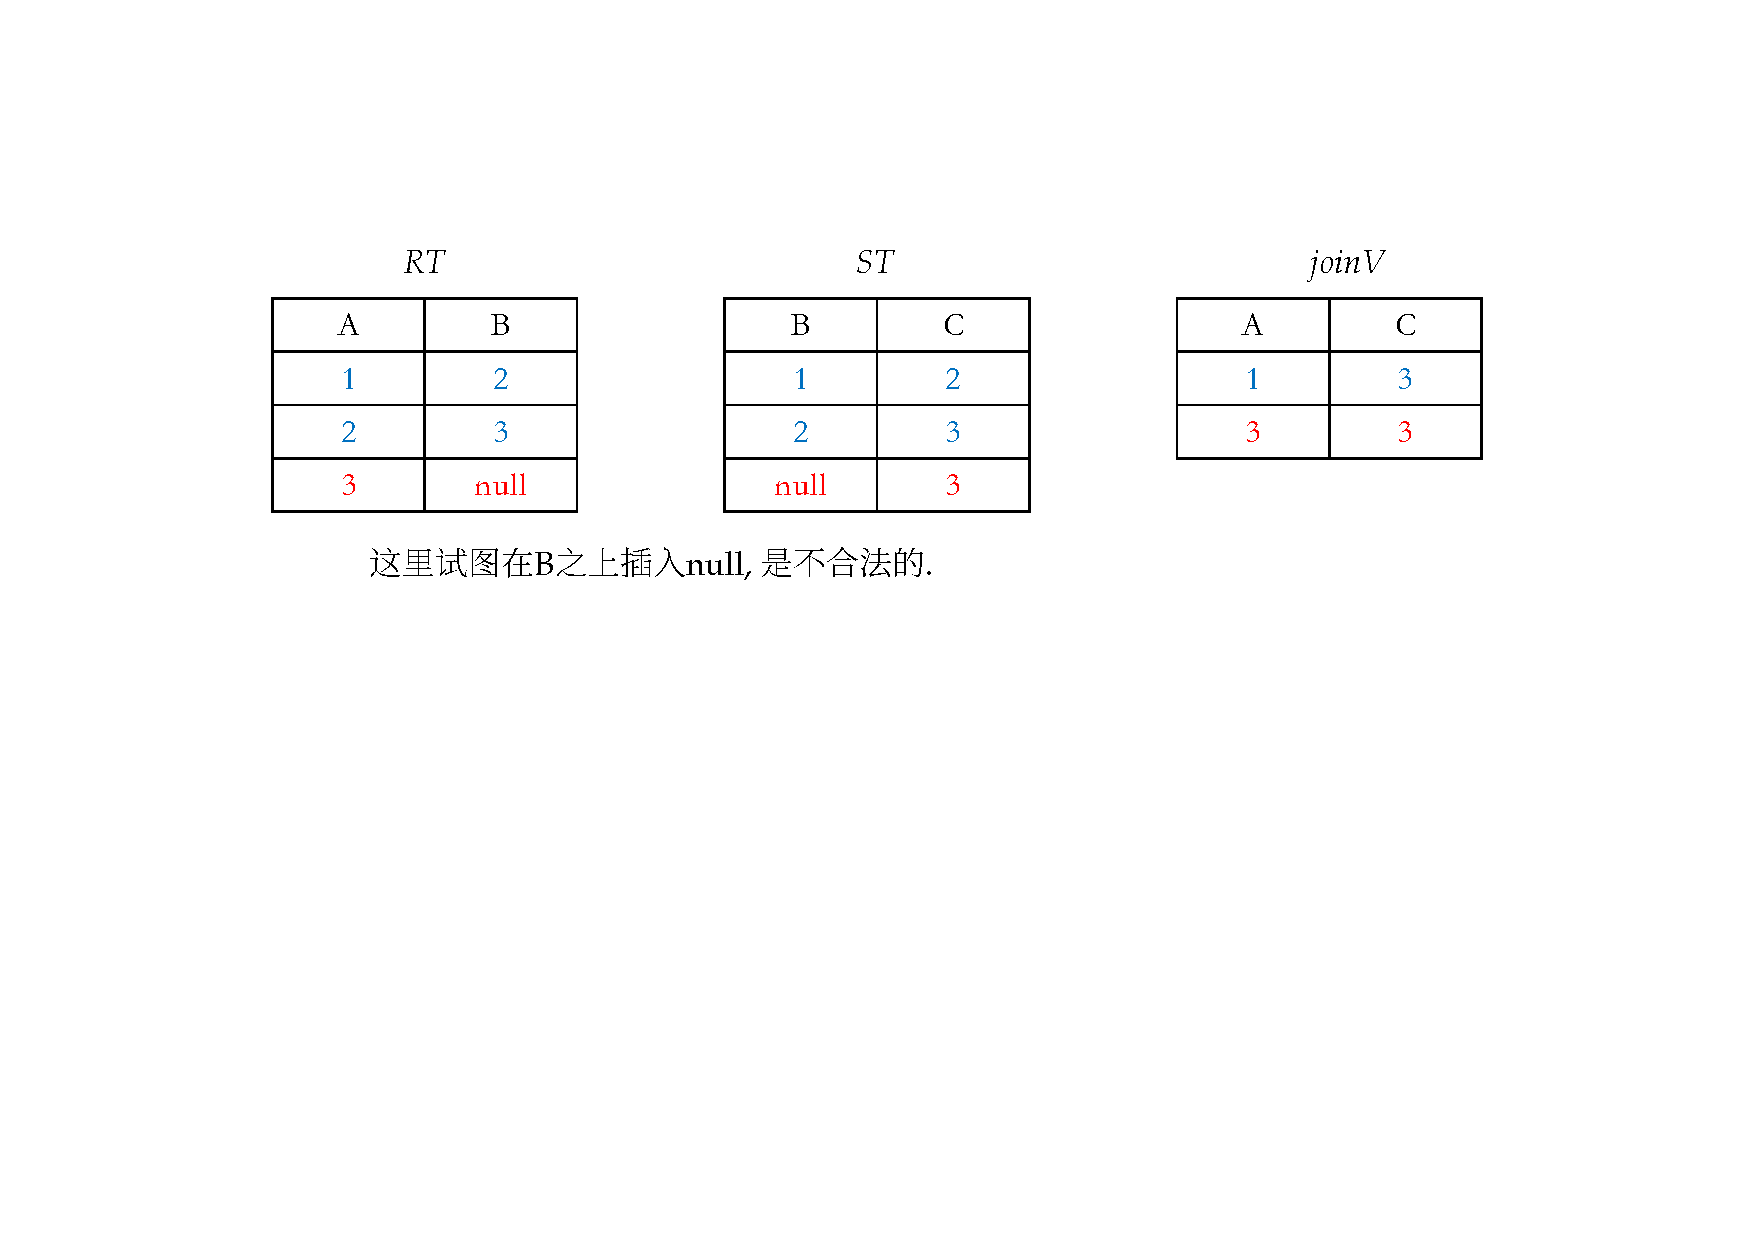
\includegraphics[width=.8\textwidth]{figure/不合法的视图更新.pdf}
    \caption{不可更新的视图: 不含连接属性}
\end{figure}

不可更新视图还包括:
\begin{itemize}
  \item select子句中的目标列包含了聚集函数;
  \item select子句中使用unique或distinct关键字;
  \item select子句中包含经算术表达式计算出来的列;
  \item from子句中包含了多个表;
  \item 包含了group by子句.
\end{itemize}

这些都是因为违反了\textbf{全关系系统准则 6: 视图更新准则}. 要存在一个算法可以无二
义地把更新要求转换为对基本表的更新序列.

\subsection{临时表和内存表}

\begin{table}[H]
\centering
\begin{tabular}{|l|l|l|}
\hline
 & 临时表 & 内存表 \\
\hline
存储 & 表结构和数据都存储在内存中 & 表结构存储在磁盘中,表数据存储在内存中 \\
\hline
会话 & 单个会话独享 & 多个会话共享 \\
\hline
断开连接 & 表结构和表数据都没了 & 表结构和表数据都存在 \\
\hline
服务重启 & 表结构和表数据都没了 & 表结构存在,表数据不存在 \\
\hline
\end{tabular}
\caption{临时表与内存表的比较}
\end{table}

\subsection{公用表表达式CTE}

\begin{lstlisting}[language=SQL]
with S-total (sno, value) as
      select sno, sum (grade)
      from SC
      group by sno
    S-total-avg(value) as
      select avg (value)
      from S-total
select sno
from S-total, S-total-avg
where S-total.value >= S-total-avg.value
\end{lstlisting}

\begin{lstlisting}[language=SQL]
values row(1,2,3), row(10,9,8)
union all
values row(-1,-2,0),row(10,29,30),row(100,20,-9)
\end{lstlisting}

\subsection{分区表}

\begin{definition}[分区表]
  把逻辑上统一的数据分割成较小的、可以独立管理的物理单元(分片)进行存储.
\end{definition}

分区表的优点:
\begin{itemize}
  \item 增强可用性;
  \item 维护方便;
  \item 均衡I/O;
  \item 改善查询性能.
\end{itemize}

一般的分区方式:
\begin{itemize}
  \item 范围分区: 根据某个属性值的范围进行分区;
  \item 散列分区: 通过分区编号将数据均匀散列到I/O设备上, 使得这些分区大小一致;
  \item 复合分区: 先使用范围分区; 再在每个分区内使用散列分区.
\end{itemize}

\section{数据查询}

开门见山: 数据查询只需要会下面的语法即可.
\begin{lstlisting}[language=SQL]
Select     <目标列>
From       <数据源表>
Where      <行过滤>
Group by   <分组>
Having     <分组过滤>
Union      <合并>
Order by   <输出排序>
Limit      <输出行数>
\end{lstlisting}

数据查询必须要经过: 笛卡尔积 $\to$ 选择 $\to$ 投影.

\begin{figure}[H]
    \centering
    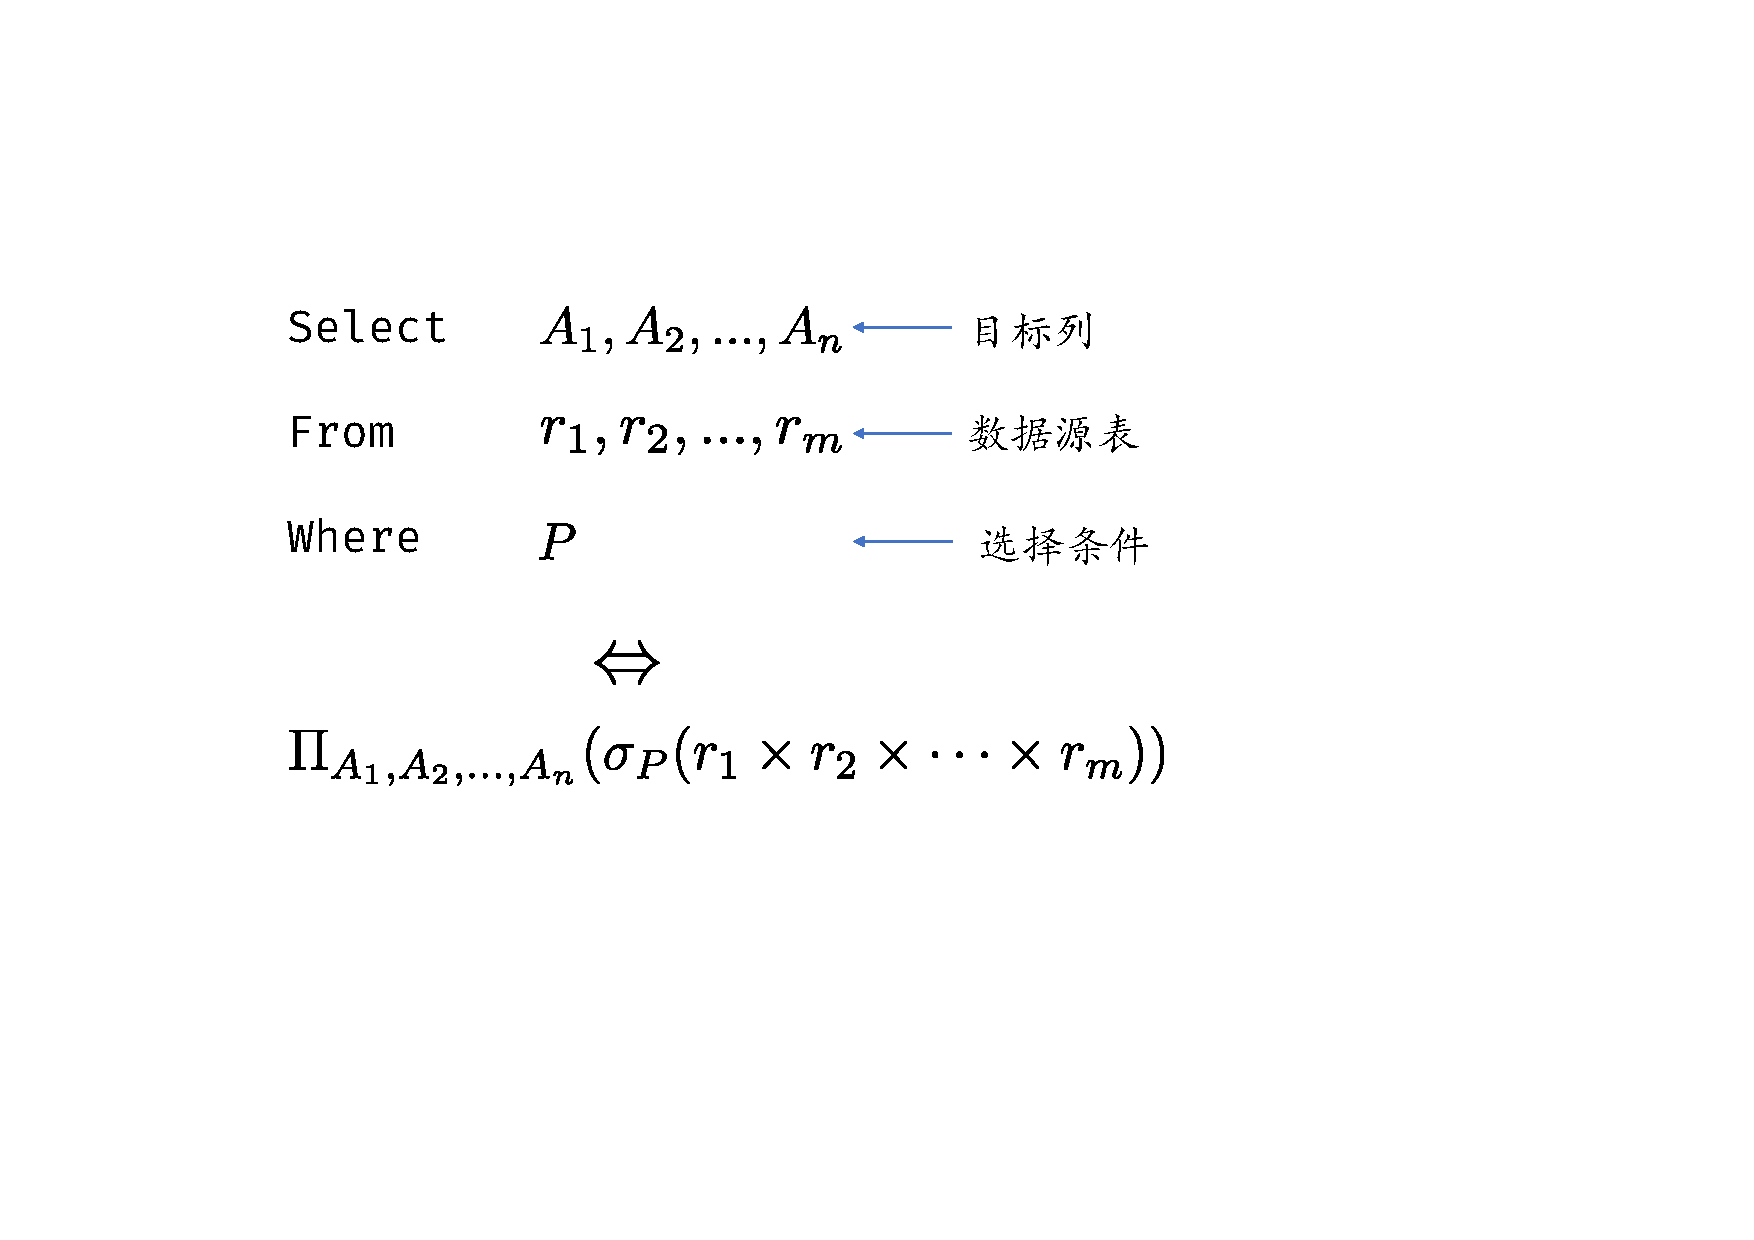
\includegraphics[width=.5\textwidth]{figure/数据查询.pdf}
    \caption{SQL查询基本结构}
\end{figure}

\begin{example}
  找出选修课程的学生姓名、课程名、成绩.
\end{example}

\textit{ 解答. }最基础的解是:
\begin{align*}
    \Pi_{sname,cname,grade} (S \bowtie SC \bowtie C).
\end{align*}
可以写成上面的三步走的形式, 如下图:
\begin{figure}[H]
    \centering
    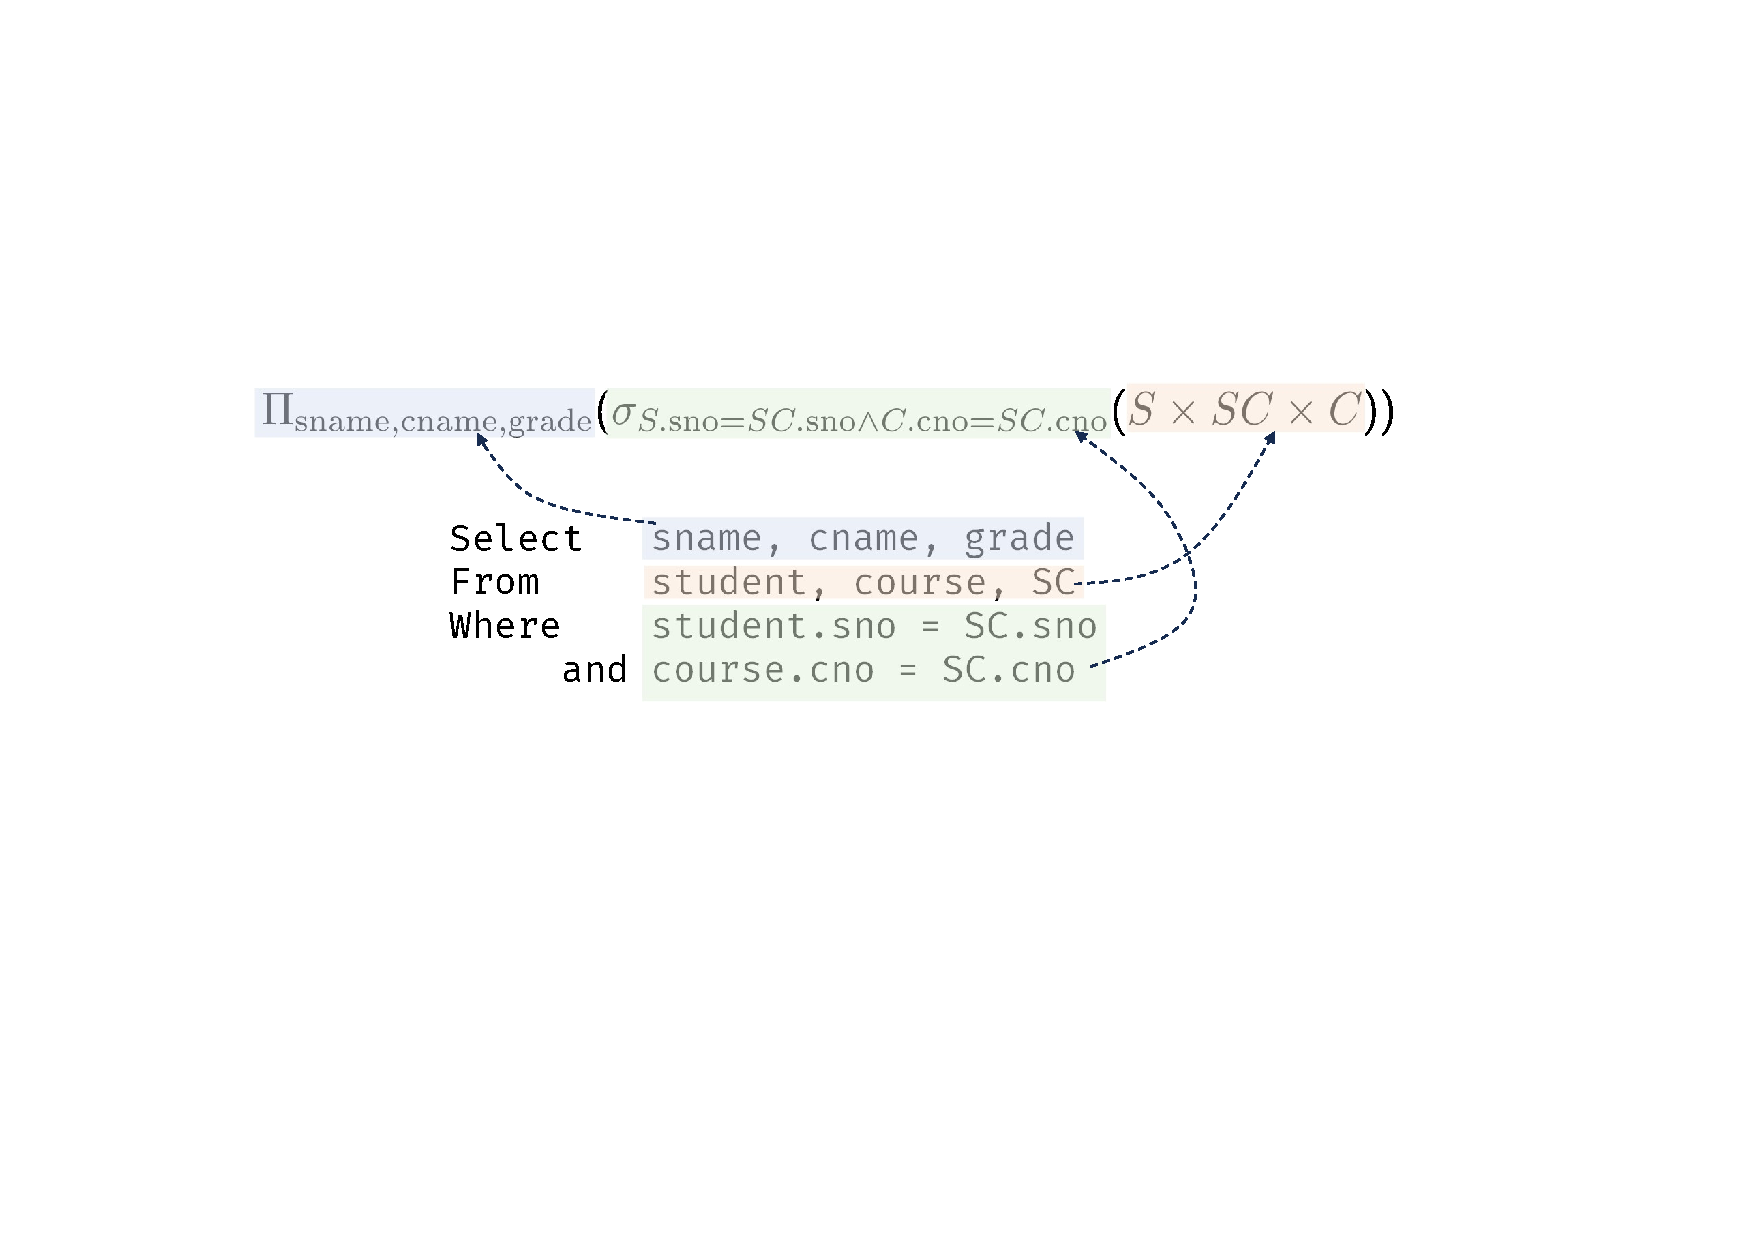
\includegraphics[width=.7\textwidth]{figure/查询例题1.pdf}
    \caption{数据查询三步走}
\end{figure}

\begin{example}
  写出与\textcolor{red}{$R(A,B) \bowtie S(B,C)$}等价的SQL.
\end{example}

\textit{ 解答. }
\begin{lstlisting}[language=SQL]
Select  A, R.B, C
From    R, S
Where   R.B = S.B
\end{lstlisting}

\begin{example}
  寻找每个学生在哪个系.
\end{example}

\textit{ 解答. }
\begin{lstlisting}[language=SQL]
Select     sname, dname
From       student, department
Where      dname = '计算机系'
      and  student.dno = department.dno
\end{lstlisting}

\begin{lstlisting}[language=SQL]
-- 给出所有学生的所有信息
select *
from student

-- 给出所有学生的姓名及出生日期
select sname, 2025-age
from student

-- 给出每个老师信息的自然语言描述
select  tname + '老师的工资是' + salary
        + ',年龄是' + age
        + ',职称是' + title
from teacher

-- 列出成绩在60~80之间的学生学号
-- 优化小窍门: 使用 between 合并两个比较谓词
select sno
from SC
where grade between 60 and 80
\end{lstlisting}

!!!注意, SQL缺省为保留重复值, 也可以用关键字 \textcolor{red}{\texttt{all}} 显式指明; 若要去掉重复行, 可以用关键字 \textcolor{red}{\texttt{distinct}} 指明.
\begin{align*}
    \Pi_A(R) = \texttt{select distinct }A\texttt{ from }R
\end{align*}

优化小窍门: 只在必要时使用 \textcolor{red}{\texttt{distinct}}.

输出顺序: \texttt{order by 列名 [asc | desc]}.
\begin{lstlisting}[language=SQL]
select *
from student
order by age asc, sname desc
-- 按照年龄升序输出学生信息, 相同年龄按照姓名降序

select tname, salary*2
from teacher
order by 2
-- 按照 输出列 的编号排序

select sname
from student
order by age
-- 排序列可以不是 输出列
\end{lstlisting}

更名运算: 可以出现在 \verb|select| 和 \verb|from| 子句中. \verb|old_name (as) new_name|.

\begin{lstlisting}[language=SQL]
select  sname '姓名',
        sex '性别',
        2025 - age '出生日期'
from student
order by 出生日期
-- 或者 order by 3

select S2.sno
from SC as S1, SC as S2
where S1.sno = 's1'
  and S1.cno = 'c1'
  and S2.cno = 'c1'
  and S1.grade < S2.grade
-- 找出比 s1 学生选修 c1 课程成绩高的学生号
\end{lstlisting}

\subsection{空值}

数据库中允许取null, 就变成了三值逻辑. true, false, unknown.
\begin{itemize}
  \item A-Mark null: 表示“未知的”. 值存在, 只是当前没有获得该信息.
  \item T-Mark null: 表示“不适用”.
\end{itemize}

\textcolor{red}{全关系系统准则 3: 空值的系统化处理. 全关系型DBMS应支持空值概念, 并用系统化的方式处理空值.}

注意: 运算中牵扯到了null, 结果都是null, 例如: \verb|null <> null| 结果为null.

注意: 空值测试. \verb|is [not] null|.
\begin{itemize}
  \item 除 \verb|is [not] null| 之外, 空值不满足任何查找条件.
  \item 如果null参与算术运算, 则该算术表达式的值为null.
  \item 如果null参与比较运算, 则结果可视为unknown.
\end{itemize}

\begin{lstlisting}[language=SQL]
select sno
from SC
where grade is null
-- 不要写成 where grade = null
\end{lstlisting}

MySQL中的空值处理函数:
\begin{itemize}
  \item \verb|isnull(expr)|: 如果 \verb|expr| 值为空, 返回1, 否则为0;
  \item \verb|ifnull(check_expr, replace_value)|: 如果 \verb|check_expr| 值为空, 返回\verb|replace_value|; 否则返回 \verb|check_expr|.
  \item \verb|nullif(expr1, expr2)|: 如果两个表达式相等则返回空值, 否则返回第一个表达式.
  \item \verb|coalesce(expr1, expr2, ... )|: 返回第一个不为null的\verb|expr|.
\end{itemize}

\begin{lstlisting}[language=SQL]
select sno, cno, ifnull (grade, 0)
from SC

select sno, cno, coalesce (grade, 0)
from SC
where coalesce (grade, 0) < 60
\end{lstlisting}

当指定 \verb|order by| 的时候, \verb|asc| 首先输出空值, \verb|desc| 最后输出空值.

如果要求首先输出空值, 然后由大到小输出非空值怎么办?
\begin{lstlisting}[language=SQL]
select  id, val,
        1 - isnull(val) as is_null
from order_null
order by is_null, val desc
\end{lstlisting}

\subsection{连接运算}

连接类型:
\begin{itemize}
  \item \verb|inner join|.
  \item \verb|left out join|.
  \item \verb|right out join|.
  \item \verb|full out join|.
\end{itemize}

\begin{lstlisting}[language=SQL, caption={不用外连接表达查询的例子}]
-- 列出所有老师的教工号、姓名、工资、所教课程号
select tno, tname, salary, cno
from teacher, TC
where teacher.tno = TC.tno
unoinselect tno, tname, salary, null
from teacher
where tno not in (select tno from TC)
\end{lstlisting}

\begin{lstlisting}[language=SQL, caption={用外连接表达查询的例子}]
-- 列出所有老师的教工号、姓名、工资、所教课程号
select tno, tname, salary, cno
from teacher left join TC
      on teacher.tno = TC.tno
\end{lstlisting}

inner join: 只保留符合连接条件的元组.
\begin{figure}[H]
    \centering
    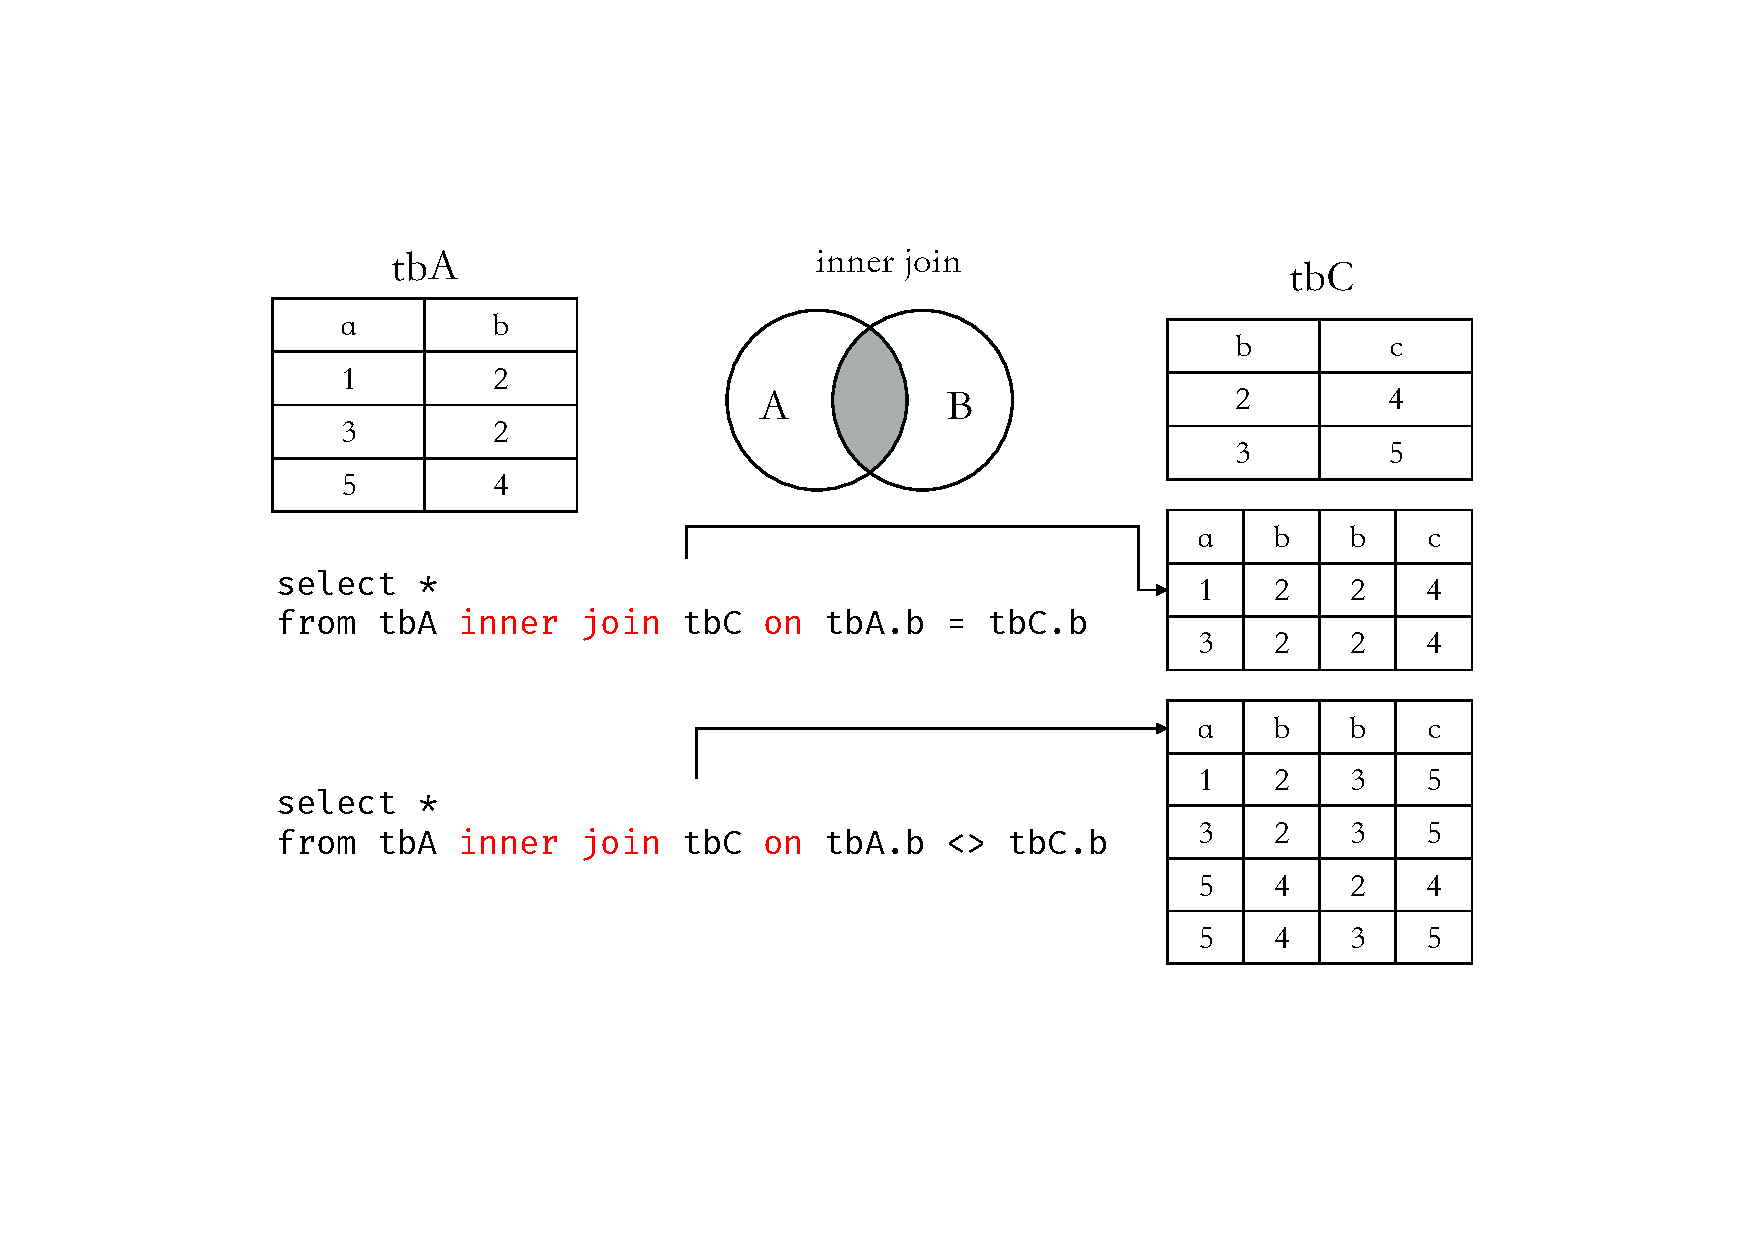
\includegraphics[width=.55\textwidth]{figure/inner_join.pdf}
    \caption{inner join示例}
\end{figure}

left join: 对于失配部分, 保留左边信息+null.

\begin{figure}[H]
    \centering
    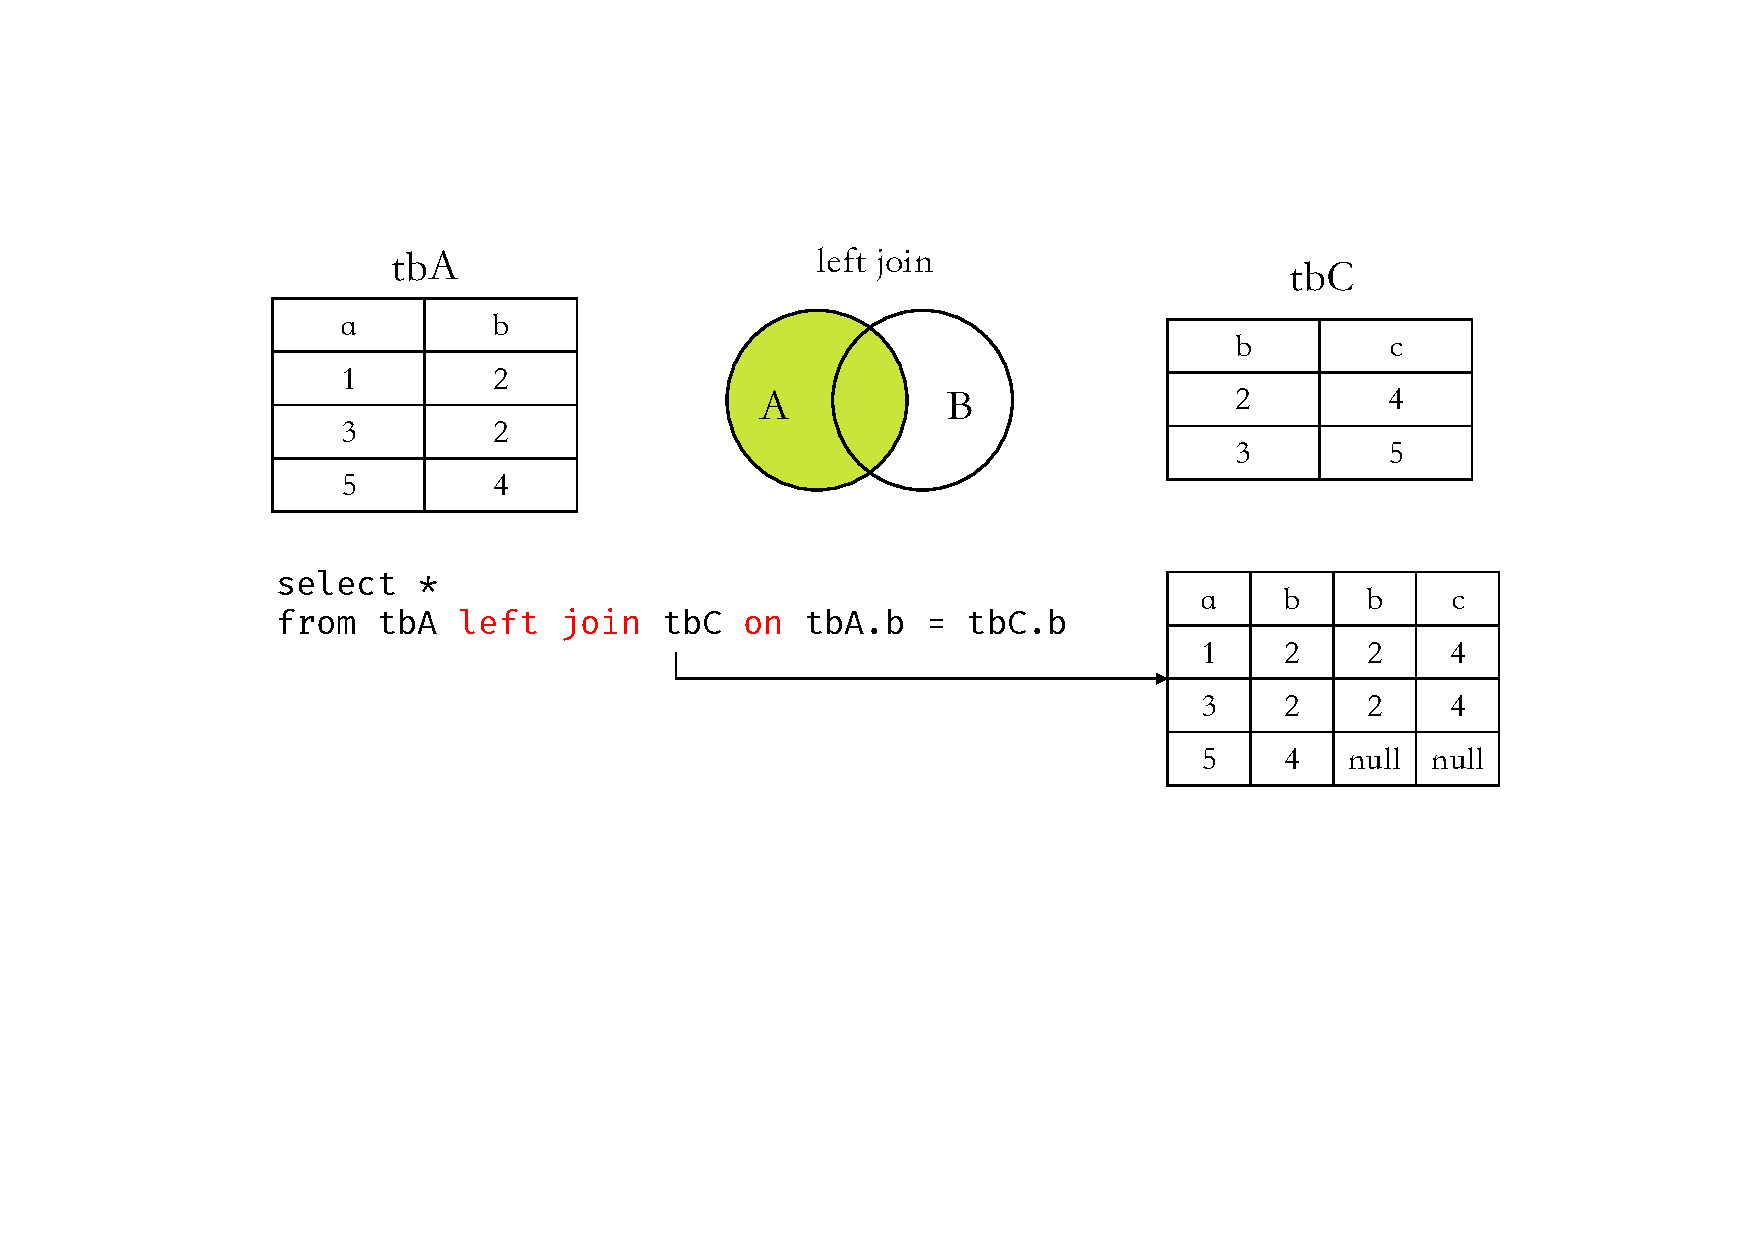
\includegraphics[width=.55\textwidth]{figure/left_join.pdf}
    \caption{left join示例}
\end{figure}

right join: 对于失配部分, 保留右边信息+(左边)null.

\begin{figure}[H]
    \centering
    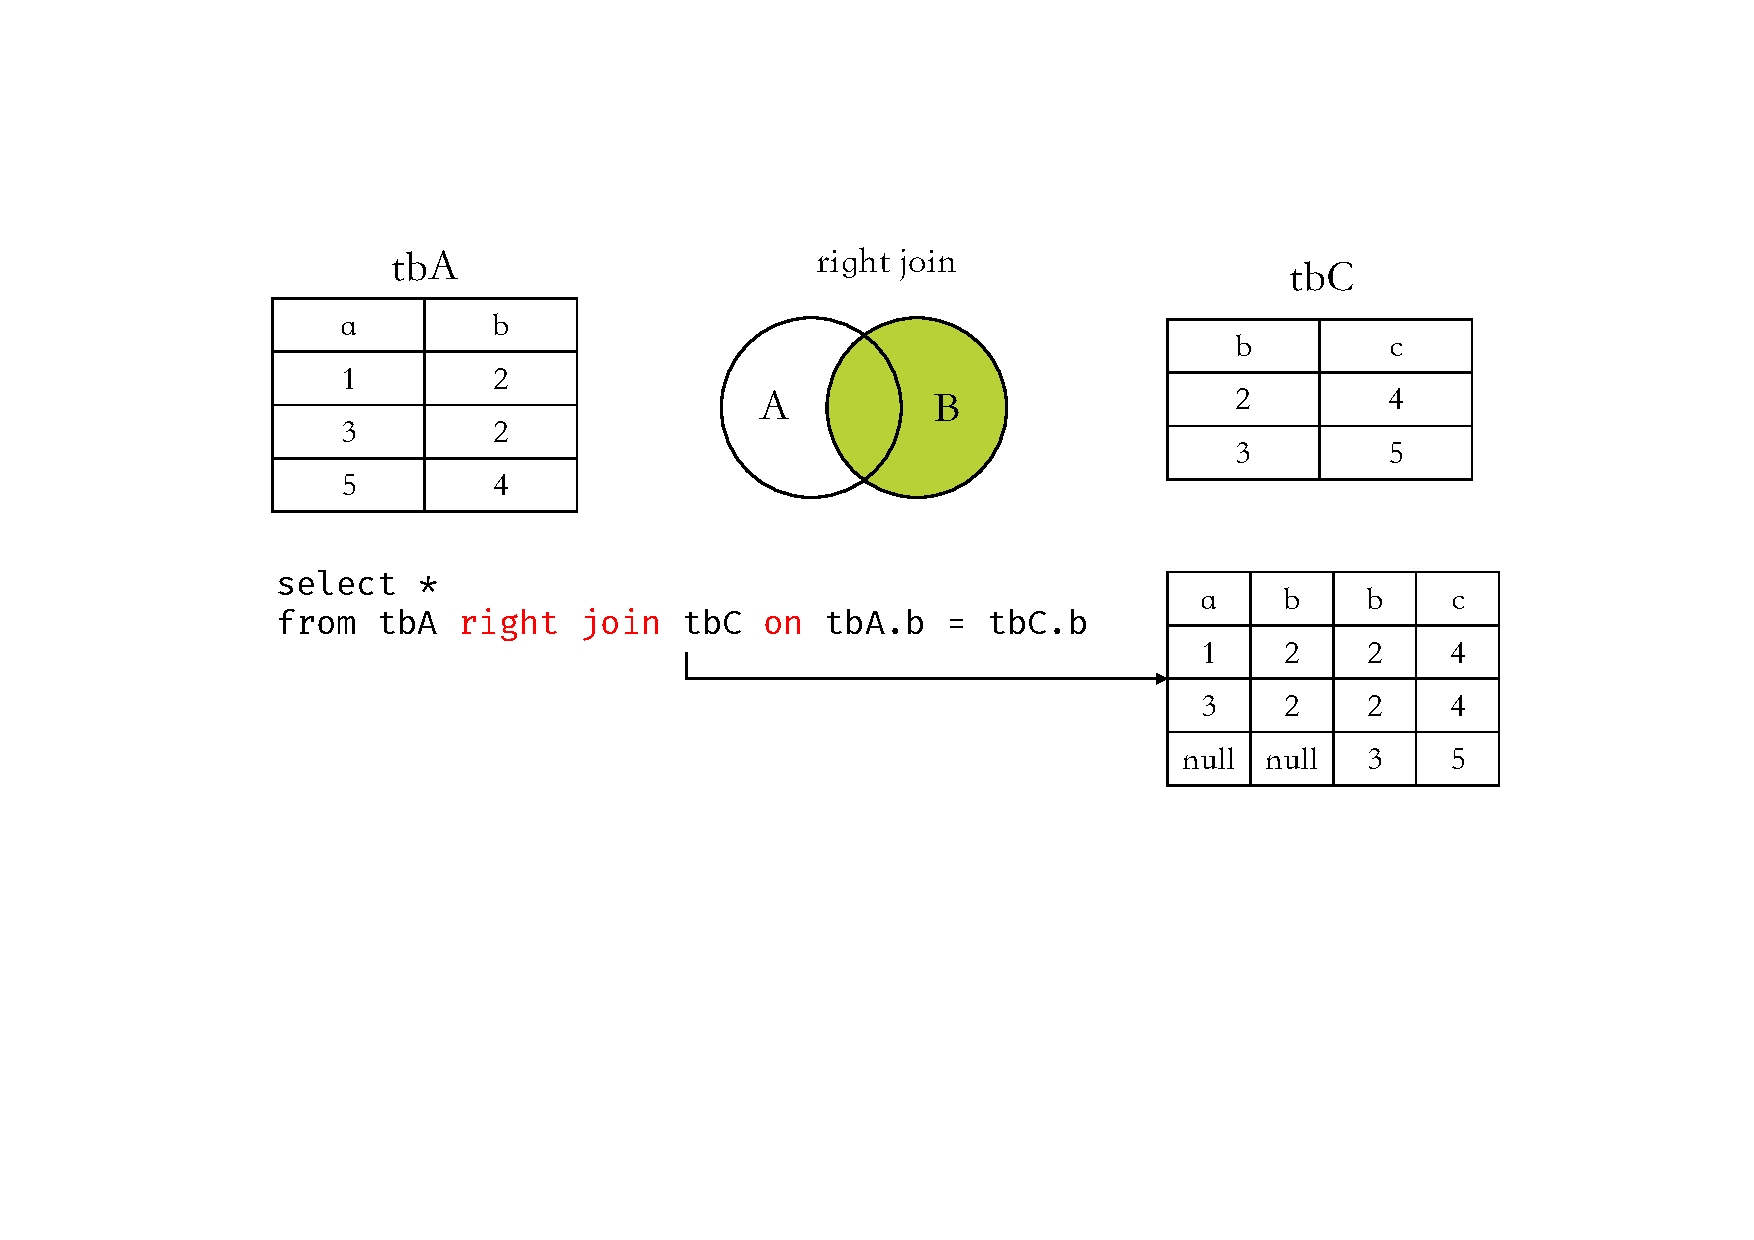
\includegraphics[width=.55\textwidth]{figure/right_join.pdf}
    \caption{right join示例}
\end{figure}

left join excluding inner join: 保留左边表中和右边失配的部分.

\begin{figure}[H]
    \centering
    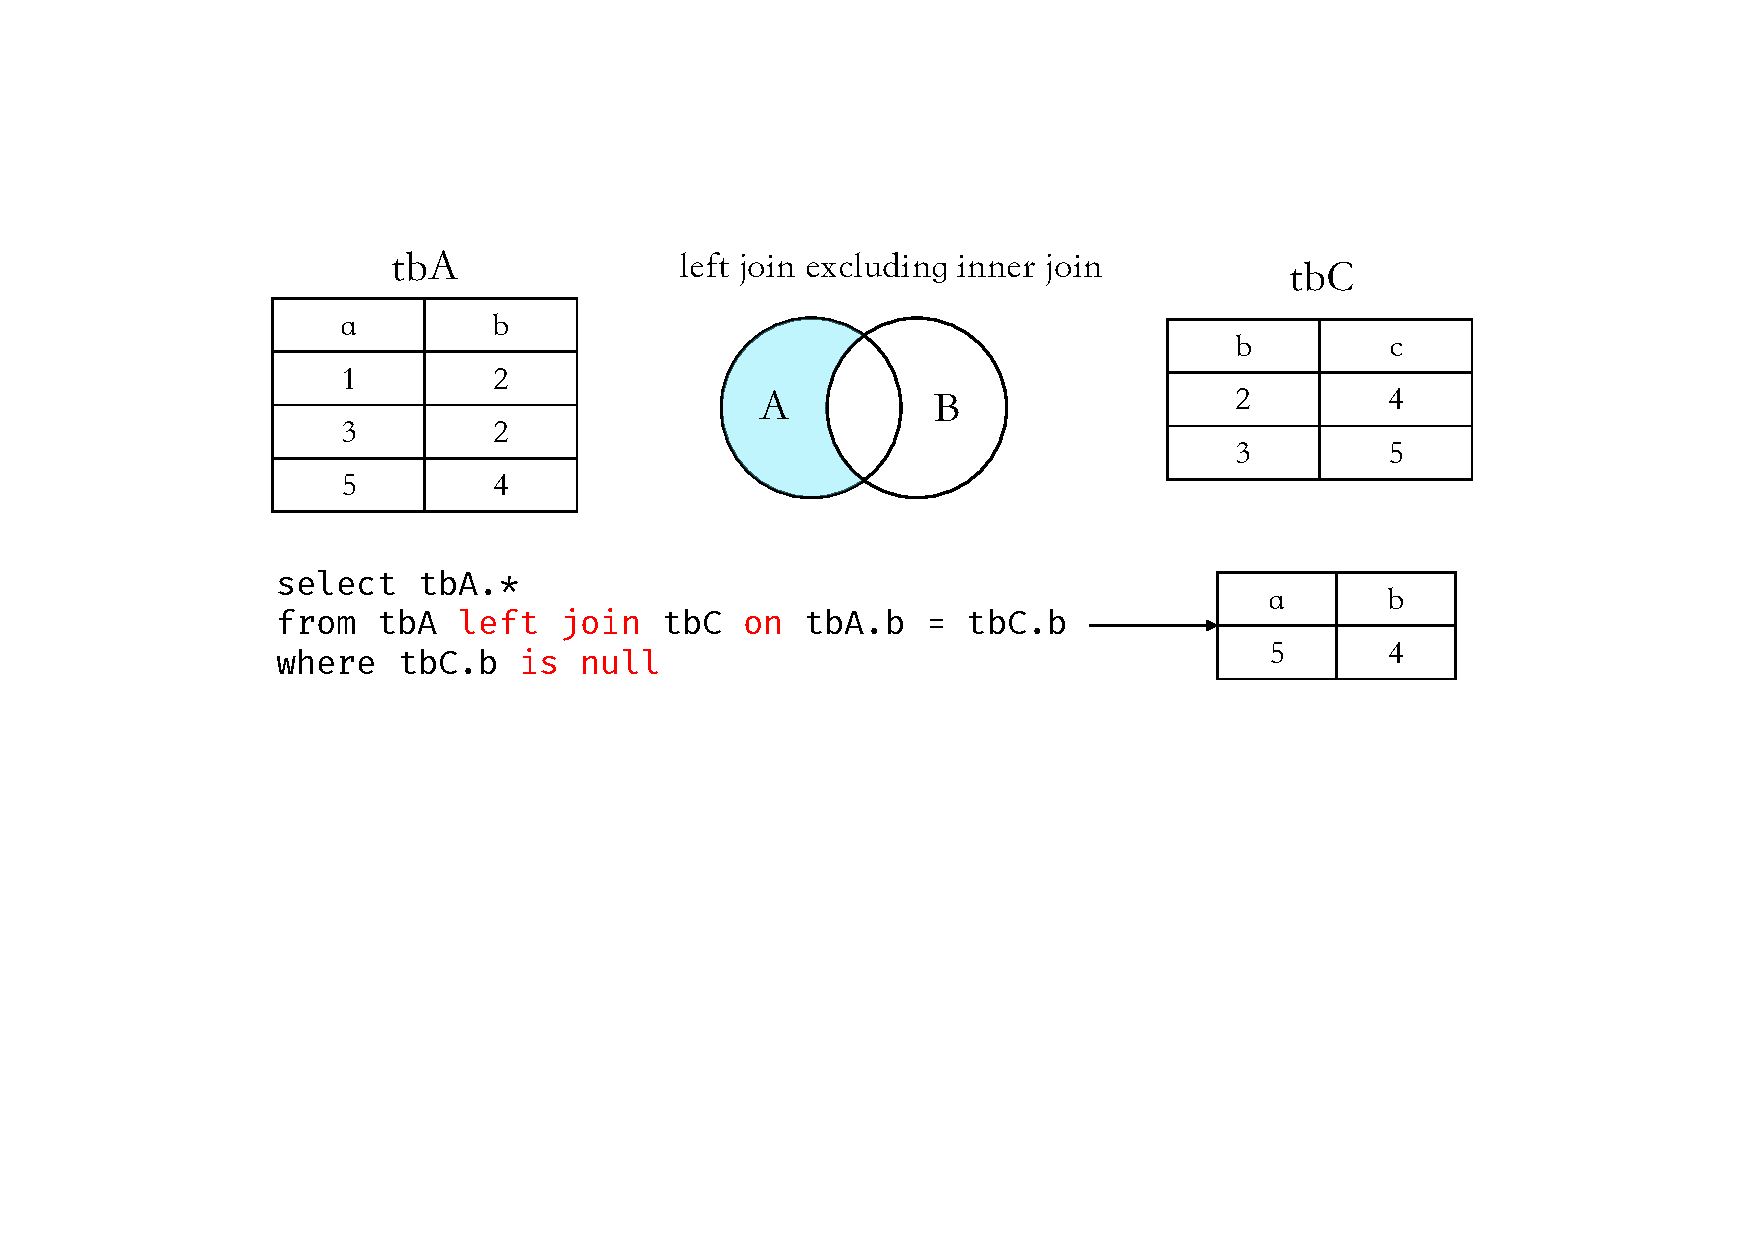
\includegraphics[width=.55\textwidth]{figure/left_join_ex_inner_join.pdf}
    \caption{left join excluding inner join}
\end{figure}

full join excluding inner join: 分别保留两边失配的部分.

\begin{figure}[H]
    \centering
    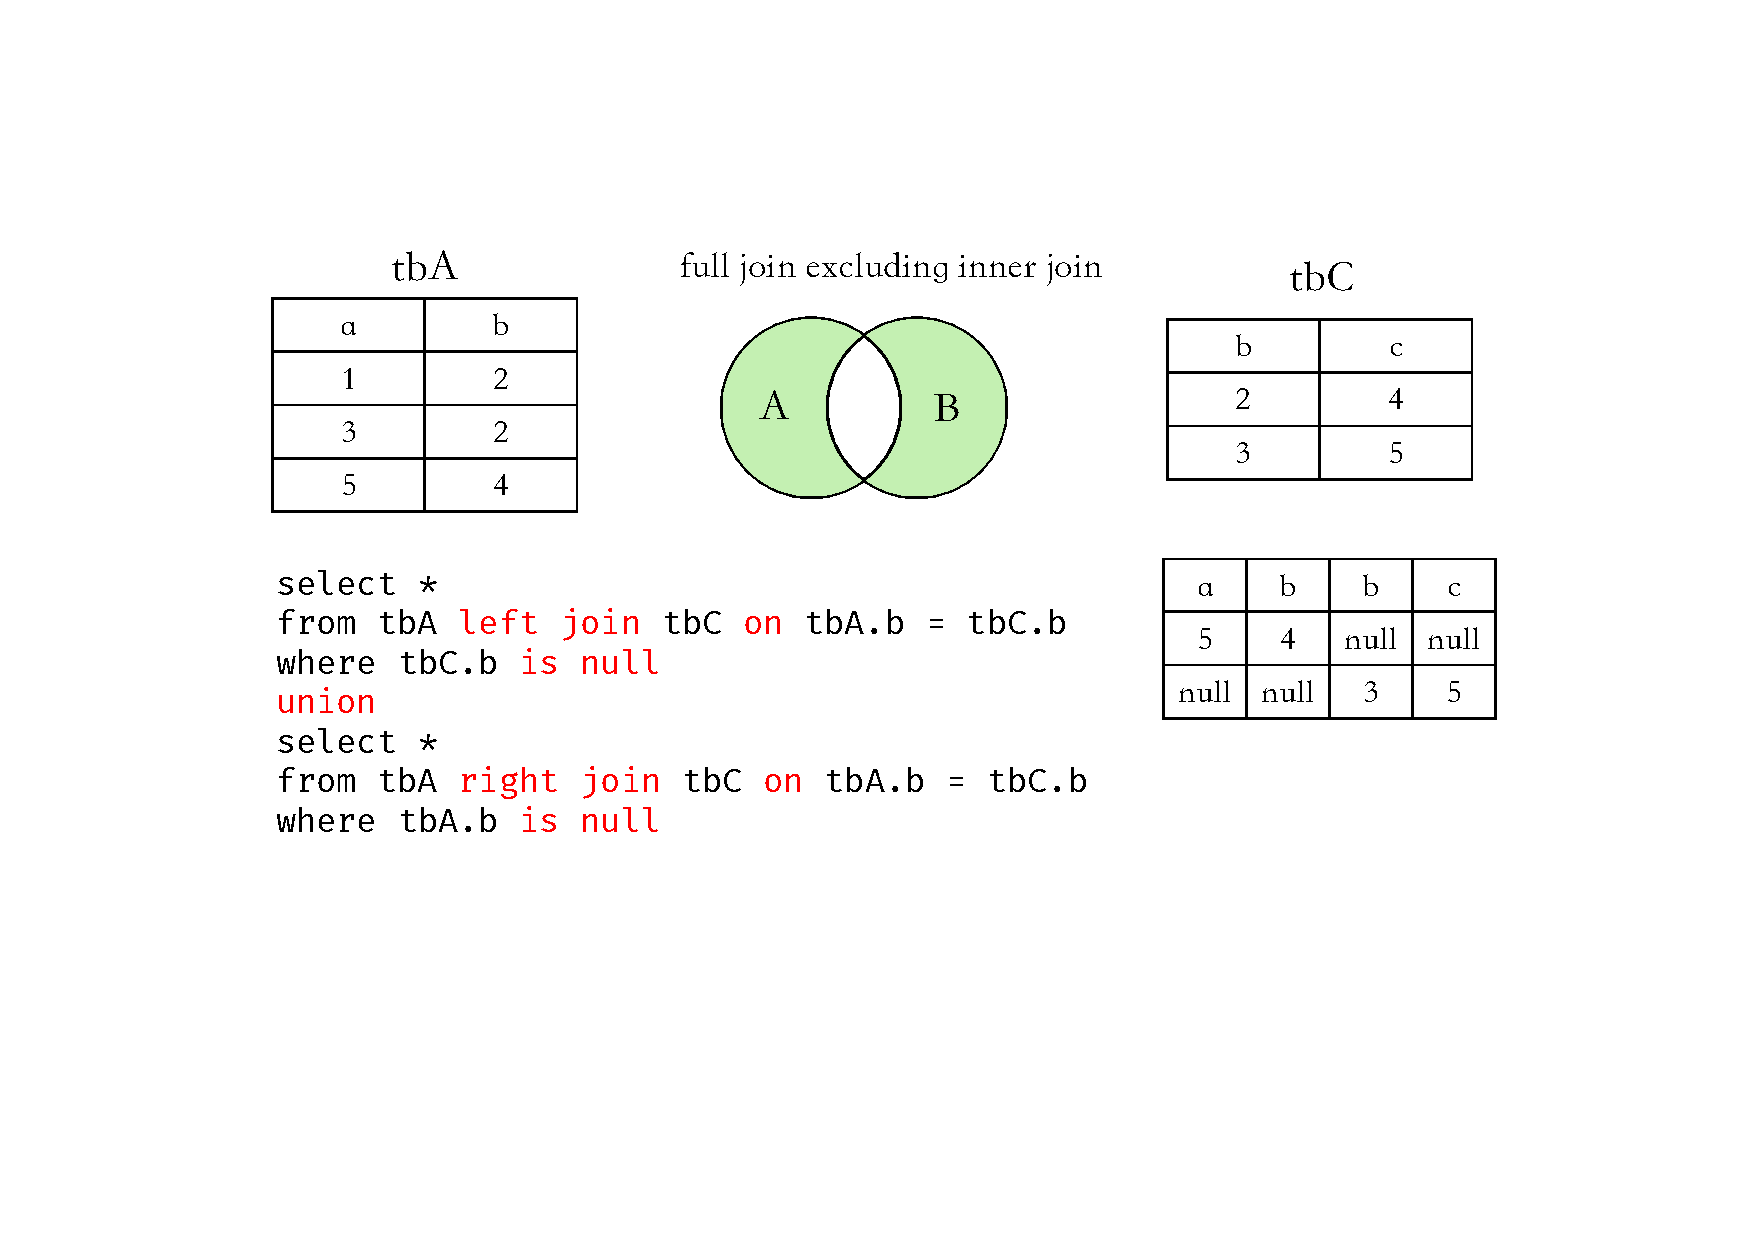
\includegraphics[width=.55\textwidth]{figure/full_join_ex.pdf}
    \caption{full join excluding inner join}
\end{figure}

cross join: \verb|(R cross join S) as T|: 两个关系的笛卡尔积.

\begin{figure}[H]
    \centering
    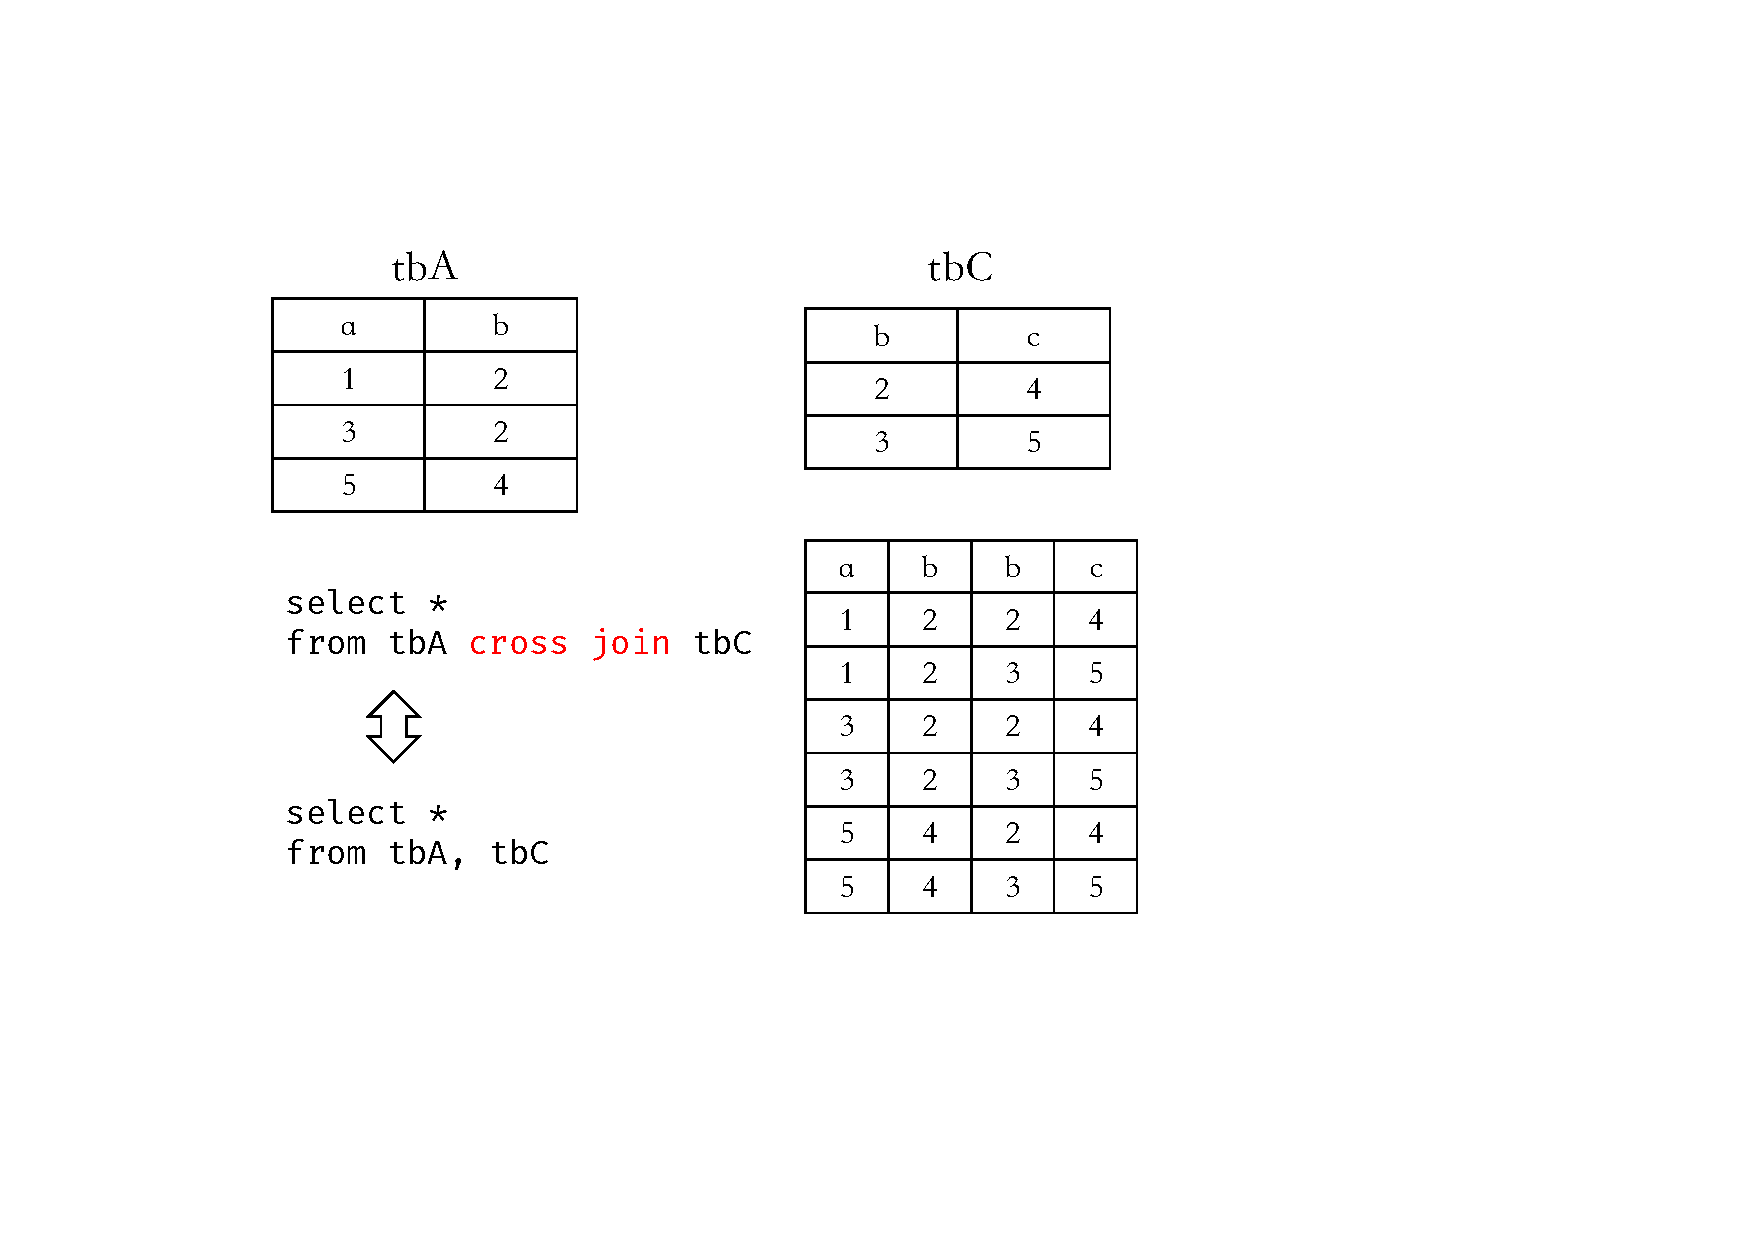
\includegraphics[width=.5\textwidth]{figure/cross_join.pdf}
    \caption{cross join}
\end{figure}

natural join: 匹配相同部分.

\begin{figure}[H]
    \centering
    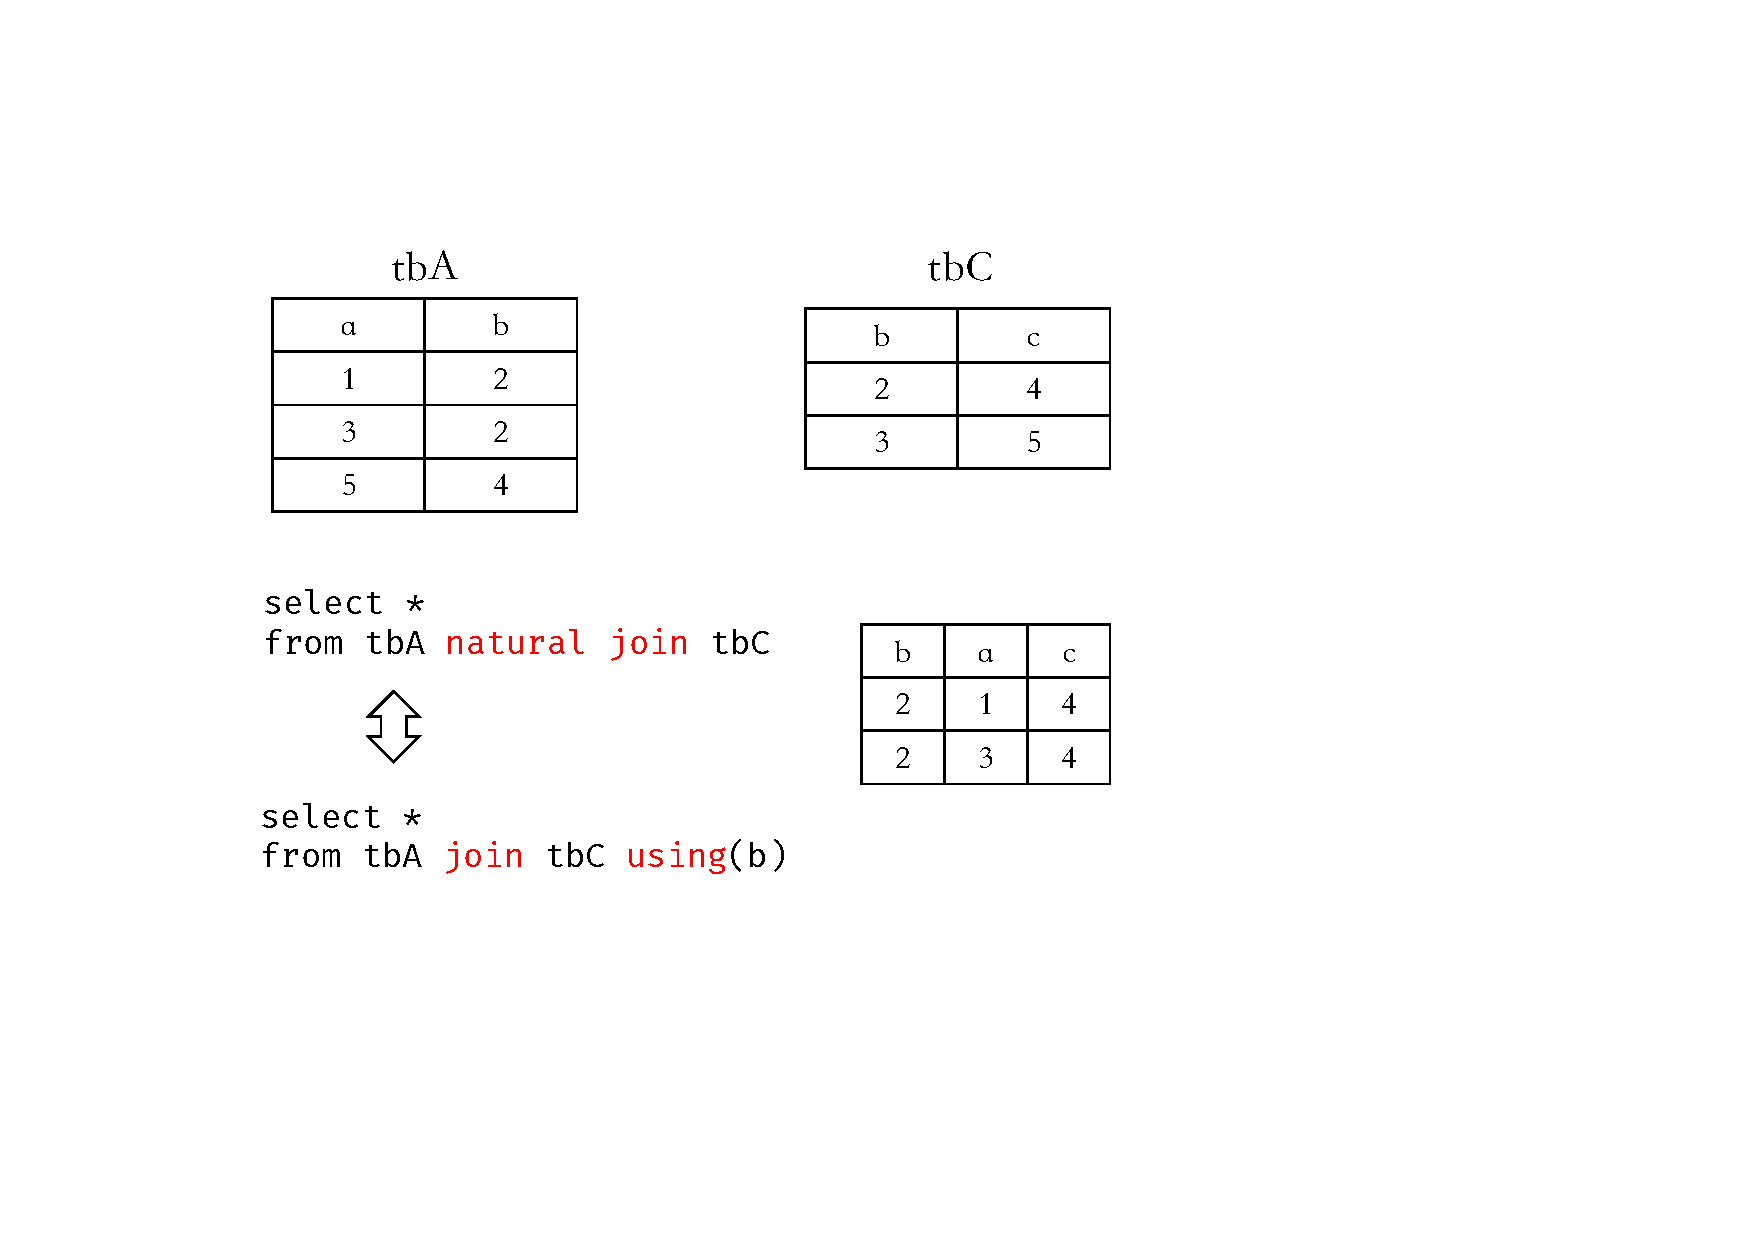
\includegraphics[width=.5\textwidth]{figure/natural_join.pdf}
    \caption{natural join}
\end{figure}

在某些数据库(如 MySQL)中, \verb|JOIN| 关键字默认等价于 \verb|INNER JOIN|, 但其他数据库(如 PostgreSQL)可能需要显式写 \verb|INNER JOIN|.

straight join:
默认情况下, MySQL 优化器会根据统计信息(如表大小、索引使用情况等)决定连接顺序. 
但在某些情况下, 优化器的选择可能不是最优的. 
此时, \verb|STRAIGHT_JOIN| 可以手动指定连接顺序, 确保左侧表作为驱动表.

\begin{lstlisting}[language=SQL, caption={多表连接}]
select *
from tbA A  inner join tbA B on A.b=B.b
            inner join tbA C on A.b=C.b

select *
from tbA A  join (tbA B, tbA C)
            on (A.b=B.b and A.b=C.b)
\end{lstlisting}

cross apply与outer apply: 提取左表中的每一行, 与右表中的所有行进行匹配.
\begin{figure}[H]
    \centering
    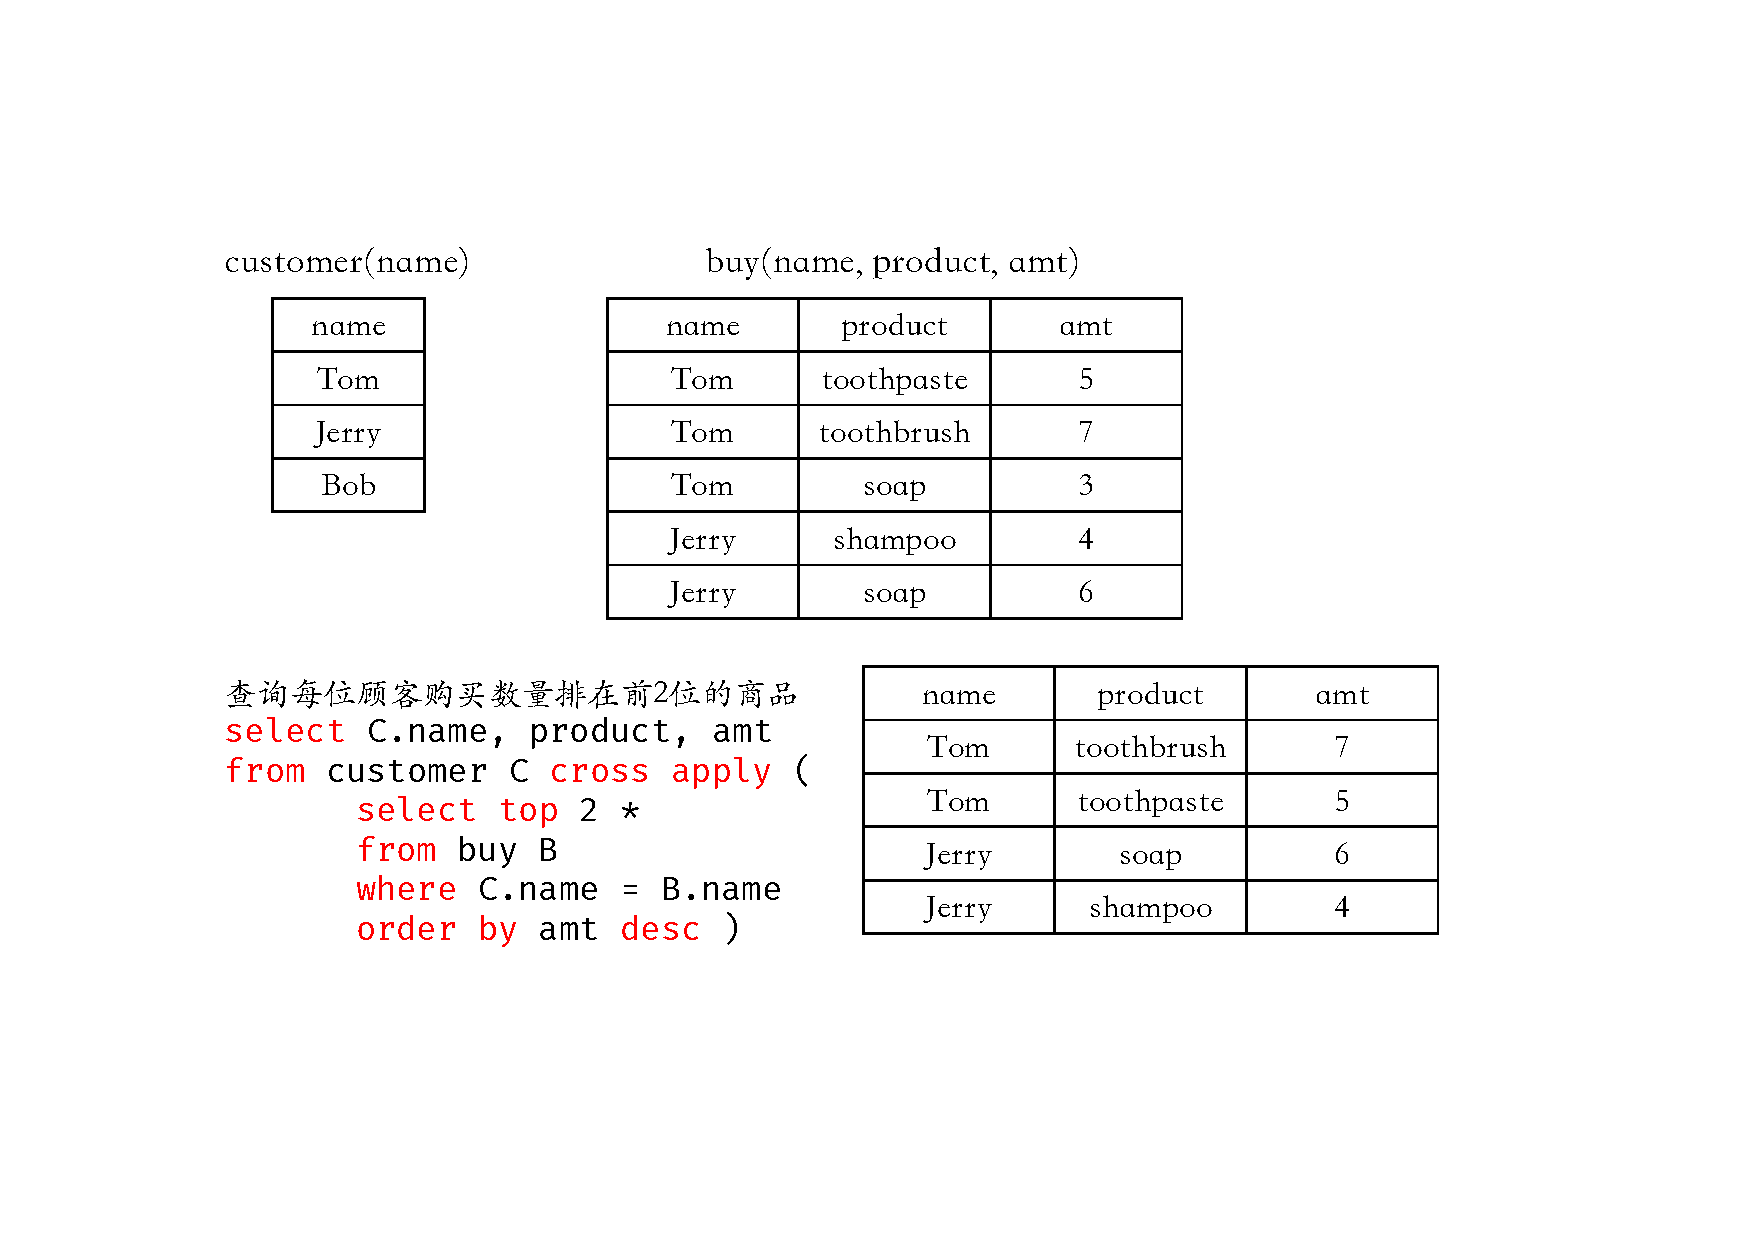
\includegraphics[width=.8\textwidth]{figure/cross_apply.pdf}
    \caption{cross apply示例}
\end{figure}

\subsection{集合运算}

\begin{itemize}
  \item 集合并: \verb|union (all)|
  \item 集合交: \verb|intersect (all)|
  \item 集合差: \verb|except (all)|
  \item 集合操作缺省去除重复元组
  \item \verb|intersect| 的优先级高于其他集合操作的优先级
  \item 加上 \verb|all| 表示当成 multi-set 来操作.
\end{itemize}

求工资大于1000或者年龄大于60的教工:
\begin{lstlisting}[language=SQL, caption={集合操作表达查询的例子}]
-- 查询 1
select tno
from teacher
where salary > 1000
union all
select tno
from teacher
where age > 60

-- 查询 2
select tno
from teacher
where salary > 1000
   or age > 60
\end{lstlisting}

上面的查询 1和查询 2等价, 但是查询 2的效率更高.

\begin{lstlisting}[language=SQL, caption={求出选修所有课程的同学}]
SELECT sno
FROM student S1
WHERE
  (
    -- 所有课程
    SELECT cno
    FROM C
    EXCEPT
    -- 除去学生选的课程
    SELECT cno
    FROM SC
    WHERE S1.sno = SC.sno
  ) IS NULL;
  -- 剩下的课程为 NULL
\end{lstlisting}

\subsection{聚集函数(Group function)}

\begin{itemize}
  \item 平均值: \verb|avg|
  \item 最小值: \verb|min|
  \item 最大值: \verb|max|
  \item 总和: \verb|sum|
  \item 记数: \verb|count|
\end{itemize}

\begin{lstlisting}[language=SQL, caption={聚集函数最容易犯的语法错误}]
select sno
from SC
where grade = max(grade)
-- Error Code: 1111. Invalid use of group function

-- 正确的使用方法
select sno
from SC
where grade = (select max(grade) from SC)
\end{lstlisting}

聚集函数处理null: \textcolor{red}{除了 \texttt{count} 之外忽略null.}

统计型聚集函数: \verb|std|, \verb|stddev|, \verb|stddev_pop|, \verb|stddev_samp|,
\verb|variance|, \verb|var_pop|, \verb|var_samp|.

\subsection{分组运算}

\verb|group by| 将表中行按指定列上值相等的原则分组, 然后在每一分组上使用聚集函数, 得到单一值.

\verb|having| 对分组进行选择, 只将聚集函数作用到满足条件的分组上.

\begin{lstlisting}[language=SQL]
-- 每门课程 所有同学的平均成绩
select avg(grade)
from SC

-- 特定同学的平均成绩
select avg(grade)
from SC
where sno = 's1'

-- 列出每个学生的最高、最低、平均成绩
select  sno,
        max(grade),
        min(grade),
        avg(grade)
from SC
group by sno
\end{lstlisting}

分组查询中各子句的顺序: where $\to$ group by $\to$ having.
\begin{lstlisting}[language=SQL]
-- 所有课程都及格了的同学的平均成绩
select sno, avg(grade)
from SC
group by sno
having min(grade) >= 60

-- 所有同学的及格了的课程的平均成绩
select sno, avg(grade)
from SC
where grade >=60
group by sno

-- 列出每一年龄组中男学生(超过50人) 的人数
select age, count(sno)
from student
where sex = 'M'
group by age
having count(*) > 50
\end{lstlisting}

\hyperlink{https://leetcode.cn/problems/sum-of-unique-elements/description/}{Leetcode 1748. 唯一元素的和}: \textit{给你一个整数数组 \texttt{nums}。数组中唯一元素是那些只出现恰好一次的元素。
请你返回 \texttt{nums} 中唯一元素的和。}

我们把原来的 \verb|nums| 数组放在表 \verb|numTb| 的 \verb|nums| 列之中.
\begin{lstlisting}[language=SQL]
select sum(nums)
from
  (select nums
   from numTb
   group by nums -- 按照 nums 的数值分组
   -- 如果组内只有一个, 说明是唯一元素
   having count(*)=1 ) tmpT
\end{lstlisting}


\begin{lstlisting}[language=SQL]
group_concat 列名
  [order by 排序列]
  [separator 分隔符]

insert into ds value  ('cs', 'bob'),
                      ('cs', 'tom'),
                      ('maths', 'mary'),
                      ('maths', 'lisa'),
                      ('maths', null);

select  dname,
        group_concat(sname)
from ds
group by dname

select  dname,
        group_concat(name order by sname)
from ds
group by dname

select  dname,
        group_concat(name order by separator ' | ')
from ds
group by dname
\end{lstlisting}

注意: $n$个属性的所有 \verb|group by|, 共有$2^n$个.

\textbf{Cube}: 其实是这样的, 假设我们$\texttt{group by }A_1,A_2,...,A_m$. 同时我们设每个属性上的Distinct的取值集合为$D_i(1\leq i\leq m)$.

那么, \verb|with cube| 会让每个属性在$\{\texttt{NULL}\}\cup D_i$上变化. 这样总共就是有:
\begin{align*}
    \prod_{i=1}^m (|D_i|+1).
\end{align*}

\begin{figure}[H]
    \centering
    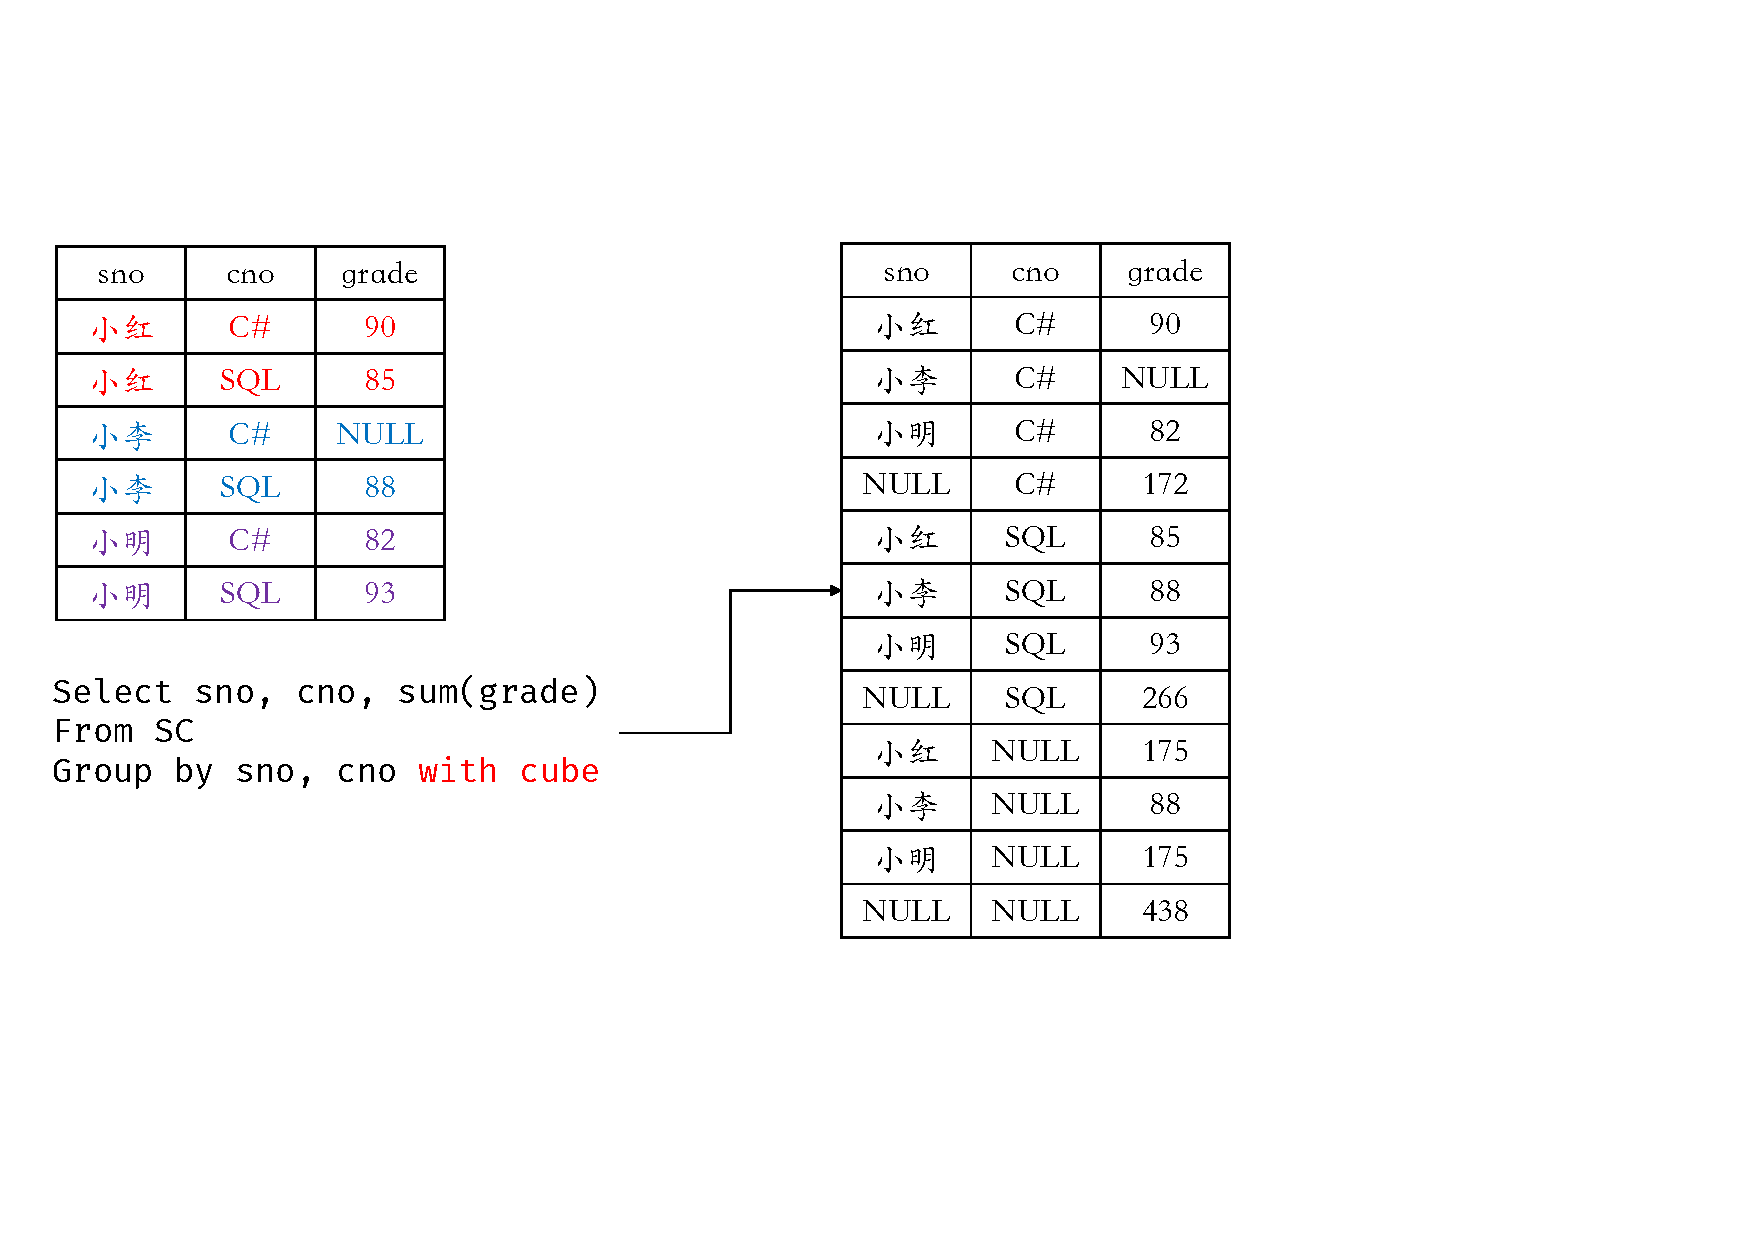
\includegraphics[width=.6\textwidth]{figure/with_cube.pdf}
    \caption{Cube示例}
\end{figure}

\begin{lstlisting}[language=SQL]
select Model, Year, Color, sum(Sales)
from car_sales
group by Model, Year, Color with cube
\end{lstlisting}

\textbf{Rollup}: 按照维度顺序统计. 例如$\texttt{group by }A_1,A_2,...,A_m$, 先不分组统计, 再按照$A_1$分组统计, 再按照$A_1,A_2$分组统计, ..., 最后按照分组$A_1,A_2,...,A_m$统计.

同时我们设每个属性上的Distinct的取值集合为$D_i(1\leq i\leq m)$.
那么Rollup产生的行数为:
\begin{align*}
    |D_1| + |D_1|\times |D_2| + |D_1|\times |D_2| \times |D_3| + \cdots + \prod_{i=1}^m |D_i| = \sum_{k=1}^m \prod_{i=1}^k |D_i|.
\end{align*}

只有 \verb|count(*)| 会把 null计入, 其他(包括 \verb|count(B)| 这样的)都不会计入.

group by将多个null行视为同一个分组.

\textbf{Grouping}: grouping是一个聚合函数, 它产生一个附加的列, 当用cube或rollup运算符添加行时, 附加
列的输出值为1, 否则为0.

\begin{lstlisting}[language=SQL]
select  if (grouping(A)=1, '汇总', '原始') grpA, A,
        if (grouping(B)=1, '汇总', '原始') grpB, B,
        count(*)
from group_null
group by A, B with rollup
\end{lstlisting}

对于grouping(A, B, C), 
\begin{itemize}
  \item 分组(A, B, C)的标识为4*0+2*0+1*0=0
  \item 分组(A, B)的标识为4*0+2*0+1*1=1
  \item 分组(A)的标识为4*0+2*1+1*1=3
  \item 分组()的标识为4*1+2*1+1*1=7
\end{itemize}

\textbf{Grouping sets}:
\begin{lstlisting}[language=SQL]
group by grouping sets
( (分组属性集1), (分组属性集2), ...(分组属性集n) )

select model, car_year, color, sum(sales)
from car_sales
group by grouping sets (
  (model, theyear),
  (model, color),
  (theyear, color),
  () )
\end{lstlisting}

\begin{align*}
&\texttt{cube}(a, b) = \texttt{grouping sets}((a, b), (a), (b), ()) \\
&\texttt{rollup}(x, y, z) = \texttt{grouping sets}((x, y, z), (x, y), (x), ()) \\
&\texttt{group by cube}(a, b), \texttt{rollup}(x, y, z) \\
&= \texttt{group by } \texttt{grouping sets}((a, b), (a), (b), ()), \texttt{grouping sets}((x, y, z), (x, y), (x), ()) \\
&= \texttt{group by grouping sets}((a, b, x, y, z), (a, b, x, y), (a, b, x), (a, b), \\
&\quad (a, x, y, z), (a, x, y), (a, x), (a), \\
&\quad (b, x, y, z), (b, x, y), (b, x), (b), \\
&\quad (x, y, z), (x, y), (x), ())
\end{align*}

\subsection{嵌套子查询}

\textbf{in子查询}. \verb|[not] in (子查询)|.

\begin{lstlisting}[language=SQL]
SELECT sname
FROM student S, SC
WHERE S.sno = SC.sno
  AND cno = 'c1';

SELECT sname
FROM student S
WHERE sno IN (
    SELECT sno
    FROM SC
    WHERE cno = 'c1'
);

-- 一般来说, 第 1 个查询更有效
\end{lstlisting}

\textbf{some/all子查询}:
\begin{itemize}
  \item 表达式 比较运算符$\theta$ some (子查询): 表达式的值至少与子查询结果中的一个值相比满足比较运算符$\theta$;
  \item 表达式 比较运算符$\theta$ all (子查询): 表达式的值与子查询结果中的所有的值相比都满足比较运算符$\theta$;
  \item =some就等价于in; $\neq$all就等价于not in.
\end{itemize}

\begin{lstlisting}[language=SQL, caption={找出平均成绩最高的学生号}]
select sno
from SC
group by sno
having avg(grade) >= all
        (select avg(grade)
        from SC
        group by sno)
\end{lstlisting}

\begin{lstlisting}[language=SQL, caption={找出每个系平均成绩最高的学生}]
select dno, S.sno
from student S, SC
where S.sno = SC.sno
group by dno, S.sno
having avg(grade) >= all
        (select avg(grade)
        from student X, SC
        where X.sno = SC.sno
        and X.dno = S.dno
        group by sno)
\end{lstlisting}

\textbf{exists子查询}: [not] exists (子查询). 判断子查询的结果集合中是否有任何元组存在.

\begin{itemize}
  \item in后的子查询与外层查询无关, 每个子查询执行一次, 称其为无关子查询.
  \item exists后的子查询与外层查询有关, 需要执行多次, 称之为相关子查询.
\end{itemize}

\begin{lstlisting}[language=SQL, caption={列出选修了c1号课程的学生姓名}]
select sname
from student S
where exists
      (select *
      from SC
      where cno = c1
      and sno = S.sno)
\end{lstlisting}

\begin{lstlisting}[language=SQL, caption={列出选修了c1号和c2号课程的学生的学号}]
select sno
from SC SC1
where SC1.cno = c1
  and exists
      (select sno
      from SC
      where cno = c2
      and sno = SC1.sno)
\end{lstlisting}

反半连接: not in, not exists.

列出没有选修课程的学生的姓名:
\begin{align*}
    \Pi_{sno}(S)-\Pi_{sno}(SC).
\end{align*}

\begin{lstlisting}[language=SQL]
select sname
from student
where sno not in
      (select sno
      from SC)

select sname
from student S
where not exists
      (select sno
      from SC
      where sno=S.sno)
\end{lstlisting}

ps. 这里后面介绍了除法 和 not exists ... not exists 的关系.

\subsection{字符串与文本操作}

LIKE 操作符:
\begin{lstlisting}[language=SQL]
SELECT * FROM table_name 
WHERE column_name LIKE pattern;
-- 查找以 "A" 开头的所有名字
SELECT * FROM users WHERE name LIKE 'A%';

-- 查找第二个字符是 "o" 的三字名字
SELECT * FROM users WHERE name LIKE '_o_';

-- 查找包含 "cat" 的名字
SELECT * FROM users WHERE name LIKE '%cat%';
\end{lstlisting}


REGEXP:
\begin{lstlisting}[language=SQL]
SELECT * FROM table_name 
WHERE column_name REGEXP pattern;

-- 查找以 "A" 开头且以 "e" 结尾的名字
SELECT * FROM users WHERE name REGEXP '^A.*e$';

-- 查找包含连续三个数字的名字
SELECT * FROM users WHERE name REGEXP '[0-9]{3}';

-- 查找格式为 "XXX-XXX-XXXX" 的电话号码
SELECT * FROM contacts WHERE phone REGEXP '^[0-9]{3}-[0-9]{3}-[0-9]{4}$';
\end{lstlisting}

\section{数据更新}

\begin{remark}
  期末考试不考!!!
\end{remark}

INSERT、DELETE、TRUNCATE、UPDATE、OUTPUT、MERGE.

\begin{lstlisting}[language=SQL]
-- 插入单条记录
INSERT INTO employees (name, age, department) 
VALUES ('John Doe', 28, 'Engineering');

-- 批量插入
INSERT INTO students (class_id, name, gender, score) 
VALUES 
  (1, '大宝', 'M', 87),
  (2, '二宝', 'M', 81);

-- 删除特定记录
DELETE FROM employees WHERE employee_id = 100;

-- 删除所有记录(危险操作!)
DELETE FROM employees;

TRUNCATE TABLE logs; -- 清空 logs 表的所有数据

-- 更新单列
UPDATE employees 
SET department = 'Senior Engineering' 
WHERE age > 30;

-- 更新多列
UPDATE customers 
SET cust_contact = 'Sam Roberts', cust_email = 'sam@toyland.com'
WHERE cust_id = '1000000006';

-- 删除记录并返回被删除的数据
DELETE FROM orders 
OUTPUT DELETED.order_id, DELETED.customer_id
WHERE order_date < '2023-01-01';

-- 合并订单数据:匹配则更新,否则插入
MERGE INTO orders AS target
USING (SELECT * FROM temp_orders) AS source
ON target.order_id = source.order_id
WHEN MATCHED THEN 
  UPDATE SET target.amount = source.amount
WHEN NOT MATCHED THEN 
  INSERT (order_id, amount) VALUES (source.order_id, source.amount);
\end{lstlisting}

\section{服务器端脚本语言}

\textcolor{red}{主要掌握游标和触发器的定义和使用!!!}

\subsection{SQL脚本语法成分}

\begin{enumerate}
    \item 局部变量: 使用 \verb|DECLARE| 声明变量, 以 \verb|@| 开头(如 \verb|@var|). 赋值可通过 \verb|SET| 或 \verb|SELECT|.
\begin{lstlisting}[language=SQL]
DECLARE @Name NVARCHAR(50) = 'Alice';
DECLARE @Counter INT = 0;
SET @Counter = 1;
SELECT @Name = Name FROM Users WHERE UserID = 1;
\end{lstlisting}
    \item 控制流:
    \begin{enumerate}
        \item 条件判断: \verb|IF...ELSE...| 和 \verb|CASE|.
\begin{lstlisting}[language=SQL]
IF @Age >= 18
    PRINT 'Adult';
ELSE
    PRINT 'Minor';

SELECT 
    Name,
    Status = CASE 
        WHEN Salary > 10000 THEN 'High'
        WHEN Salary > 5000 THEN 'Medium'
        ELSE 'Low'
    END
FROM Employees;
\end{lstlisting}
        \item 循环结构: \verb|WHILE| 和 \verb|LOOP ... LEAVE / ITERATE|.
\begin{lstlisting}[language=SQL]
DECLARE @i INT = 1;
WHILE @i <= 5
BEGIN
    PRINT 'Iteration ' + CAST(@i AS NVARCHAR);
    SET @i += 1;
END
\end{lstlisting}
    \end{enumerate}
      \item 异常处理, 使用 \verb|TRY...CATCH|.
\begin{lstlisting}
BEGIN TRY
    UPDATE Accounts SET Balance = Balance - 100 WHERE AccountID = 1;
    UPDATE Accounts SET Balance = Balance + 100 WHERE AccountID = 2;
END TRY
BEGIN CATCH
    ROLLBACK;
    PRINT 'Error: ' + ERROR_MESSAGE();
END CATCH
\end{lstlisting}
  \item 游标(Cursor).
\begin{lstlisting}[language=SQL]
-- 1. 声明游标
DECLARE employee_cursor CURSOR FOR
SELECT EmployeeID, Name FROM Employees WHERE Department = 'Sales';

-- 2. 打开游标
OPEN employee_cursor;

-- 3. 声明变量存储提取的数据
DECLARE @EmpID INT, @Name NVARCHAR(50);

-- 4. 提取数据并处理
FETCH NEXT FROM employee_cursor INTO @EmpID, @Name;
WHILE @@FETCH_STATUS = 0
BEGIN
    PRINT 'Employee ID: ' + CAST(@EmpID AS NVARCHAR) + ', Name: ' + @Name;
    FETCH NEXT FROM employee_cursor INTO @EmpID, @Name;
END

-- 5. 关闭游标
CLOSE employee_cursor;

-- 6. 释放游标
FREE employee_cursor;
\end{lstlisting}
  \item 动态 SQL.
\begin{lstlisting}[language=SQL]
DECLARE @SQL NVARCHAR(MAX);
SET @SQL = 'SELECT * FROM Users WHERE Name = ''Alice''';
EXEC(@SQL);

DECLARE @SQL NVARCHAR(MAX), @Name NVARCHAR(50) = 'Alice';
SET @SQL = N'SELECT * FROM Users WHERE Name = @Name';
EXEC sp_executesql @SQL, N'@Name NVARCHAR(50)', @Name;
\end{lstlisting}
\end{enumerate}

\subsection{服务器端 SQL 脚本形式}

\begin{enumerate}
    \item 批处理(Batch).一组 SQL 语句的集合, 通过 \verb|GO| 分隔.
\begin{lstlisting}[language=SQL]
-- GO 是 SQL Server 的批处理分隔符(非 SQL 标准)
DECLARE @Msg NVARCHAR(50) = 'Hello';
PRINT @Msg;
GO
PRINT @Msg; -- 错误:@Msg 作用域仅在第一个批处理中
\end{lstlisting}
    \item 存储过程(Stored Procedure): 预编译的 SQL 代码块, 可接受输入/输出参数.
\begin{lstlisting}[language=SQL]
CREATE PROCEDURE usp_GetEmployee
    @ID INT
AS
BEGIN
    SELECT * FROM Employees WHERE EmployeeID = @ID;
END

EXEC usp_GetEmployee @ID = 1;
\end{lstlisting}
  \item 函数(Function): 标量函数(返回单个值), 表值函数(返回表结果集).
\begin{lstlisting}
CREATE FUNCTION dbo.GetAge(@DOB DATE)
RETURNS INT
AS
BEGIN
    RETURN DATEDIFF(YEAR, @DOB, GETDATE());
END

SELECT dbo.GetAge('2000-01-01');

CREATE FUNCTION dbo.GetEmployeesByDept(@Dept NVARCHAR(50))
RETURNS TABLE
AS
RETURN SELECT * FROM Employees WHERE Department = @Dept;

SELECT * FROM dbo.GetEmployeesByDept('Sales');
\end{lstlisting}
  \item 触发器(Trigger): 在表的 \verb|INSERT|, \verb|UPDATE|, \verb|DELETE| 操作前后自动执行的代码.
\begin{lstlisting}[language=SQL]
CREATE TRIGGER trg_AuditLog
ON Employees
AFTER UPDATE
AS
BEGIN
    INSERT INTO AuditLog (Action, Timestamp)
    VALUES ('Update', GETDATE());
END
\end{lstlisting}
\end{enumerate}
